\documentclass[11pt,twocolumn]{article}

\usepackage[margin=0.75in]{geometry}
\usepackage{graphicx}
\usepackage{booktabs}
\usepackage{amsmath}
\usepackage{hyperref}
\usepackage{xcolor}
\usepackage{float}
\usepackage{enumitem}
\usepackage{caption}
\usepackage{subcaption}
\usepackage{multirow}
\usepackage{array}
\usepackage{tabularx}
\usepackage{fancyhdr}
\usepackage[numbers]{natbib}
\usepackage{algorithm}
\usepackage{algpseudocode}

\graphicspath{{charts/}}

\hypersetup{
    colorlinks=true,
    linkcolor=blue!60!black,
    citecolor=blue!60!black,
    urlcolor=blue!60!black,
}

\pagestyle{fancy}
\fancyhf{}
\fancyhead[L]{\small MealPlanAgent}
\fancyhead[R]{\small CMPE 258}
\fancyfoot[C]{\thepage}

\title{\textbf{MealPlanAgent: An AI-Powered Meal Planning System\\with Hybrid RAG and Multi-Model Evaluation}}
\author{Parth Patel\\
\small Department of Computer Engineering\\
\small San Jose State University\\
\small \texttt{parth.patel@sjsu.edu}}
\date{May 2026}

\begin{document}
\maketitle

% ============================================================
\begin{abstract}
We present MealPlanAgent, a vertical AI application that generates personalized weekly meal plans by combining large language models with a hybrid retrieval-augmented generation pipeline. The system implements a Planner-Executor-Critic agent architecture with five specialized tools, a three-way hybrid retriever (BM25 + dense vector + knowledge graph re-ranking), and a stateful memory system that learns user preferences across sessions. We evaluate the system across three LLMs (Llama~3.3~70B, Llama~3.2~3B, and Granite~3.1~2B) on a 60-case structured test set, measuring constraint satisfaction, allergy safety, citation accuracy, and latency. Our retrieval ablation study over 330 ground truth queries demonstrates that the full hybrid configuration achieves the best performance (P@5=0.655, MRR=0.688, NDCG@10=0.438), with statistically significant improvements over single-component configurations. Hyperparameter sensitivity analysis and bootstrap confidence intervals provide rigorous evidence for our design choices. A comprehensive test suite of 146 unit and integration tests verifies component-level correctness.
\end{abstract}

% ============================================================
\section{Introduction}

Meal planning is a daily task that involves balancing nutritional requirements, dietary restrictions, time constraints, ingredient availability, and personal preferences. While recipe recommendation systems exist, they typically address only one dimension (e.g., ingredient matching) without providing end-to-end meal plans with grocery lists, nutrition summaries, and safety verification.

We address this gap with MealPlanAgent, an LLM-powered agent system that:
\begin{enumerate}[nosep]
    \item Takes natural language meal requests and converts them to structured constraints
    \item Retrieves relevant recipes using a 3-way hybrid RAG pipeline
    \item Plans, executes, and verifies meal plans through a Planner-Executor-Critic loop
    \item Learns user preferences through a stateful memory system
    \item Produces actionable outputs: meal plans with citations, categorized grocery lists, nutrition summaries, and budget estimates
\end{enumerate}

\noindent\textbf{Contributions:}
\begin{itemize}[nosep]
    \item A hybrid retrieval pipeline combining BM25, dense vectors, and knowledge graph re-ranking with reciprocal rank fusion
    \item A Planner-Executor-Critic agent architecture with five tools and retry-based self-correction
    \item A write-summarize-retrieve memory system backed by SQLite
    \item Comprehensive evaluation: multi-model comparison on 60 test cases, retrieval ablation over 6 configurations, hyperparameter sensitivity analysis, and statistical significance testing
    \item A Streamlit web application with structured logging and safety guardrails
\end{itemize}

% ============================================================
\section{Related Work}

\textbf{Retrieval-Augmented Generation.} RAG~\cite{lewis2020rag} augments LLM generation with retrieved context from external knowledge bases. Extensions include GraphRAG~\cite{edge2024graphrag}, which incorporates knowledge graph structure, and hybrid retrieval approaches combining sparse (BM25) and dense retrieval~\cite{chen2024bge}. Our system uses a three-way fusion of BM25, vector similarity, and knowledge graph re-ranking.

\textbf{Agentic AI Systems.} Tool-using LLM agents~\cite{schick2023toolformer} extend language models with external capabilities. The ReAct paradigm~\cite{yao2022react} interleaves reasoning and action. Our Planner-Executor-Critic architecture separates planning (LLM), execution (deterministic tools), and verification (rule-based critic) for reliability.

\textbf{Meal Planning and Recipe Recommendation.} Prior work on recipe recommendation includes content-based filtering~\cite{freyne2010recommending}, collaborative filtering, and knowledge graph approaches. Our system goes beyond recommendation to provide complete meal plans with safety verification and grocery logistics.

% ============================================================
\section{System Architecture}

\subsection{Overview}

Figure~\ref{fig:architecture} illustrates the system architecture. User constraints flow through four stages: (1) natural language parsing, (2) LLM-based planning with few-shot examples, (3) tool-based execution with hybrid RAG retrieval, and (4) rule-based critic verification with up to 2 retry cycles.

\begin{figure}[H]
\centering
\fbox{\parbox{0.9\columnwidth}{\small\ttfamily
User Input $\rightarrow$ [NL Parser] \\
\hspace*{1em}$\rightarrow$ [Planner + Few-Shot + Memory] \\
\hspace*{1em}$\rightarrow$ [Executor: 5 Tools] \\
\hspace*{2em}recipe\_search (Hybrid RAG) \\
\hspace*{2em}allergy\_checker \\
\hspace*{2em}nutrition \\
\hspace*{2em}grocery\_list \\
\hspace*{2em}budget\_estimator \\
\hspace*{1em}$\rightarrow$ [Critic: Rule-Based Verify] \\
\hspace*{1em}$\rightarrow$ [Memory: Write + Summarize] \\
\hspace*{1em}$\rightarrow$ Output (UI / PDF)
}}
\caption{MealPlanAgent pipeline architecture.}
\label{fig:architecture}
\end{figure}

\subsection{Planner-Executor-Critic Agent Loop}

The \textbf{Planner} receives user constraints, few-shot examples (3 curated examples for output format consistency), and optional memory context from past sessions. It calls the LLM to produce a structured JSON plan specifying meal queries, allergens, and execution steps.

The \textbf{Executor} dispatches tool calls sequentially: recipe search for each meal slot, allergy checking, nutrition computation, grocery list aggregation, and budget estimation. All tool calls are logged via a structured JSONL logger.

The \textbf{Critic} performs five deterministic rule-based checks: (1) at least one recipe returned, (2) no allergy violations, (3) all recipes have citations, (4) no duplicate recipes, (5) valid cooking schedule entries. If any check fails, the critic generates fix instructions that are fed back to the Planner for re-planning (up to 2 retries).

\begin{algorithm}[H]
\caption{Planner-Executor-Critic Loop}
\begin{algorithmic}[1]
\State $plan \gets \text{Planner}(constraints, fewshot, memory)$
\For{$attempt = 0$ to $\text{MAX\_RETRIES}$}
    \State $result \gets \text{Executor}(plan, constraints)$
    \State $critic \gets \text{Critic}(result)$
    \If{$critic.valid$}
        \State \textbf{break}
    \EndIf
    \State $plan \gets \text{Planner}(constraints + critic.fixes)$
\EndFor
\State $\text{Memory.write}(result)$
\State \Return $result$
\end{algorithmic}
\end{algorithm}

\subsection{Hybrid RAG Pipeline}

Our retrieval system combines three complementary approaches:

\textbf{BM25 (Sparse Retrieval):} Keyword-based retrieval using Okapi BM25 scoring over recipe text. Effective for exact ingredient and tag matches.

\textbf{Dense Vector Retrieval:} Semantic similarity search using sentence-transformers/all-MiniLM-L6-v2 embeddings (384 dimensions, 22M parameters) stored in ChromaDB. Captures semantic relationships that keyword search misses.

\textbf{Knowledge Graph Re-ranking:} A NetworkX graph connecting recipes to ingredients and tags via \texttt{HAS\_INGREDIENT} and \texttt{HAS\_TAG} edges. Re-ranks retrieval results by boosting recipes that share graph neighbors with user preferences.

Results from BM25 and vector retrieval are merged using Reciprocal Rank Fusion (RRF):
\begin{equation}
\text{RRF}(d) = \sum_{r \in R} \frac{1}{k + \text{rank}_r(d)}
\end{equation}
where $k=60$ is the fusion constant and $R$ is the set of ranked lists. The KG then applies a preference-based boost:
\begin{equation}
\text{score}'(d) = \text{score}(d) + w \cdot \frac{|\text{neighbors}(d) \cap \text{prefs}|}{|\text{prefs}|}
\end{equation}
where $w=0.1$ is the boost weight.

\subsection{Knowledge Graph Construction}

The knowledge graph is built from 9,999 recipes with three node types:
\begin{itemize}[nosep]
    \item \textbf{Recipe nodes} (9,999): one per recipe with metadata
    \item \textbf{Ingredient nodes} (5,332): normalized ingredient names
    \item \textbf{Tag nodes} (476): cuisine, dietary, and cooking tags
\end{itemize}
The graph contains 270,466 edges with a density of 0.002. The average recipe degree is 27.0 (ingredients + tags), and the average ingredient degree is 16.9 (recipes using it). Figure~\ref{fig:kg_analysis} shows the structural analysis.

\begin{figure}[H]
\centering
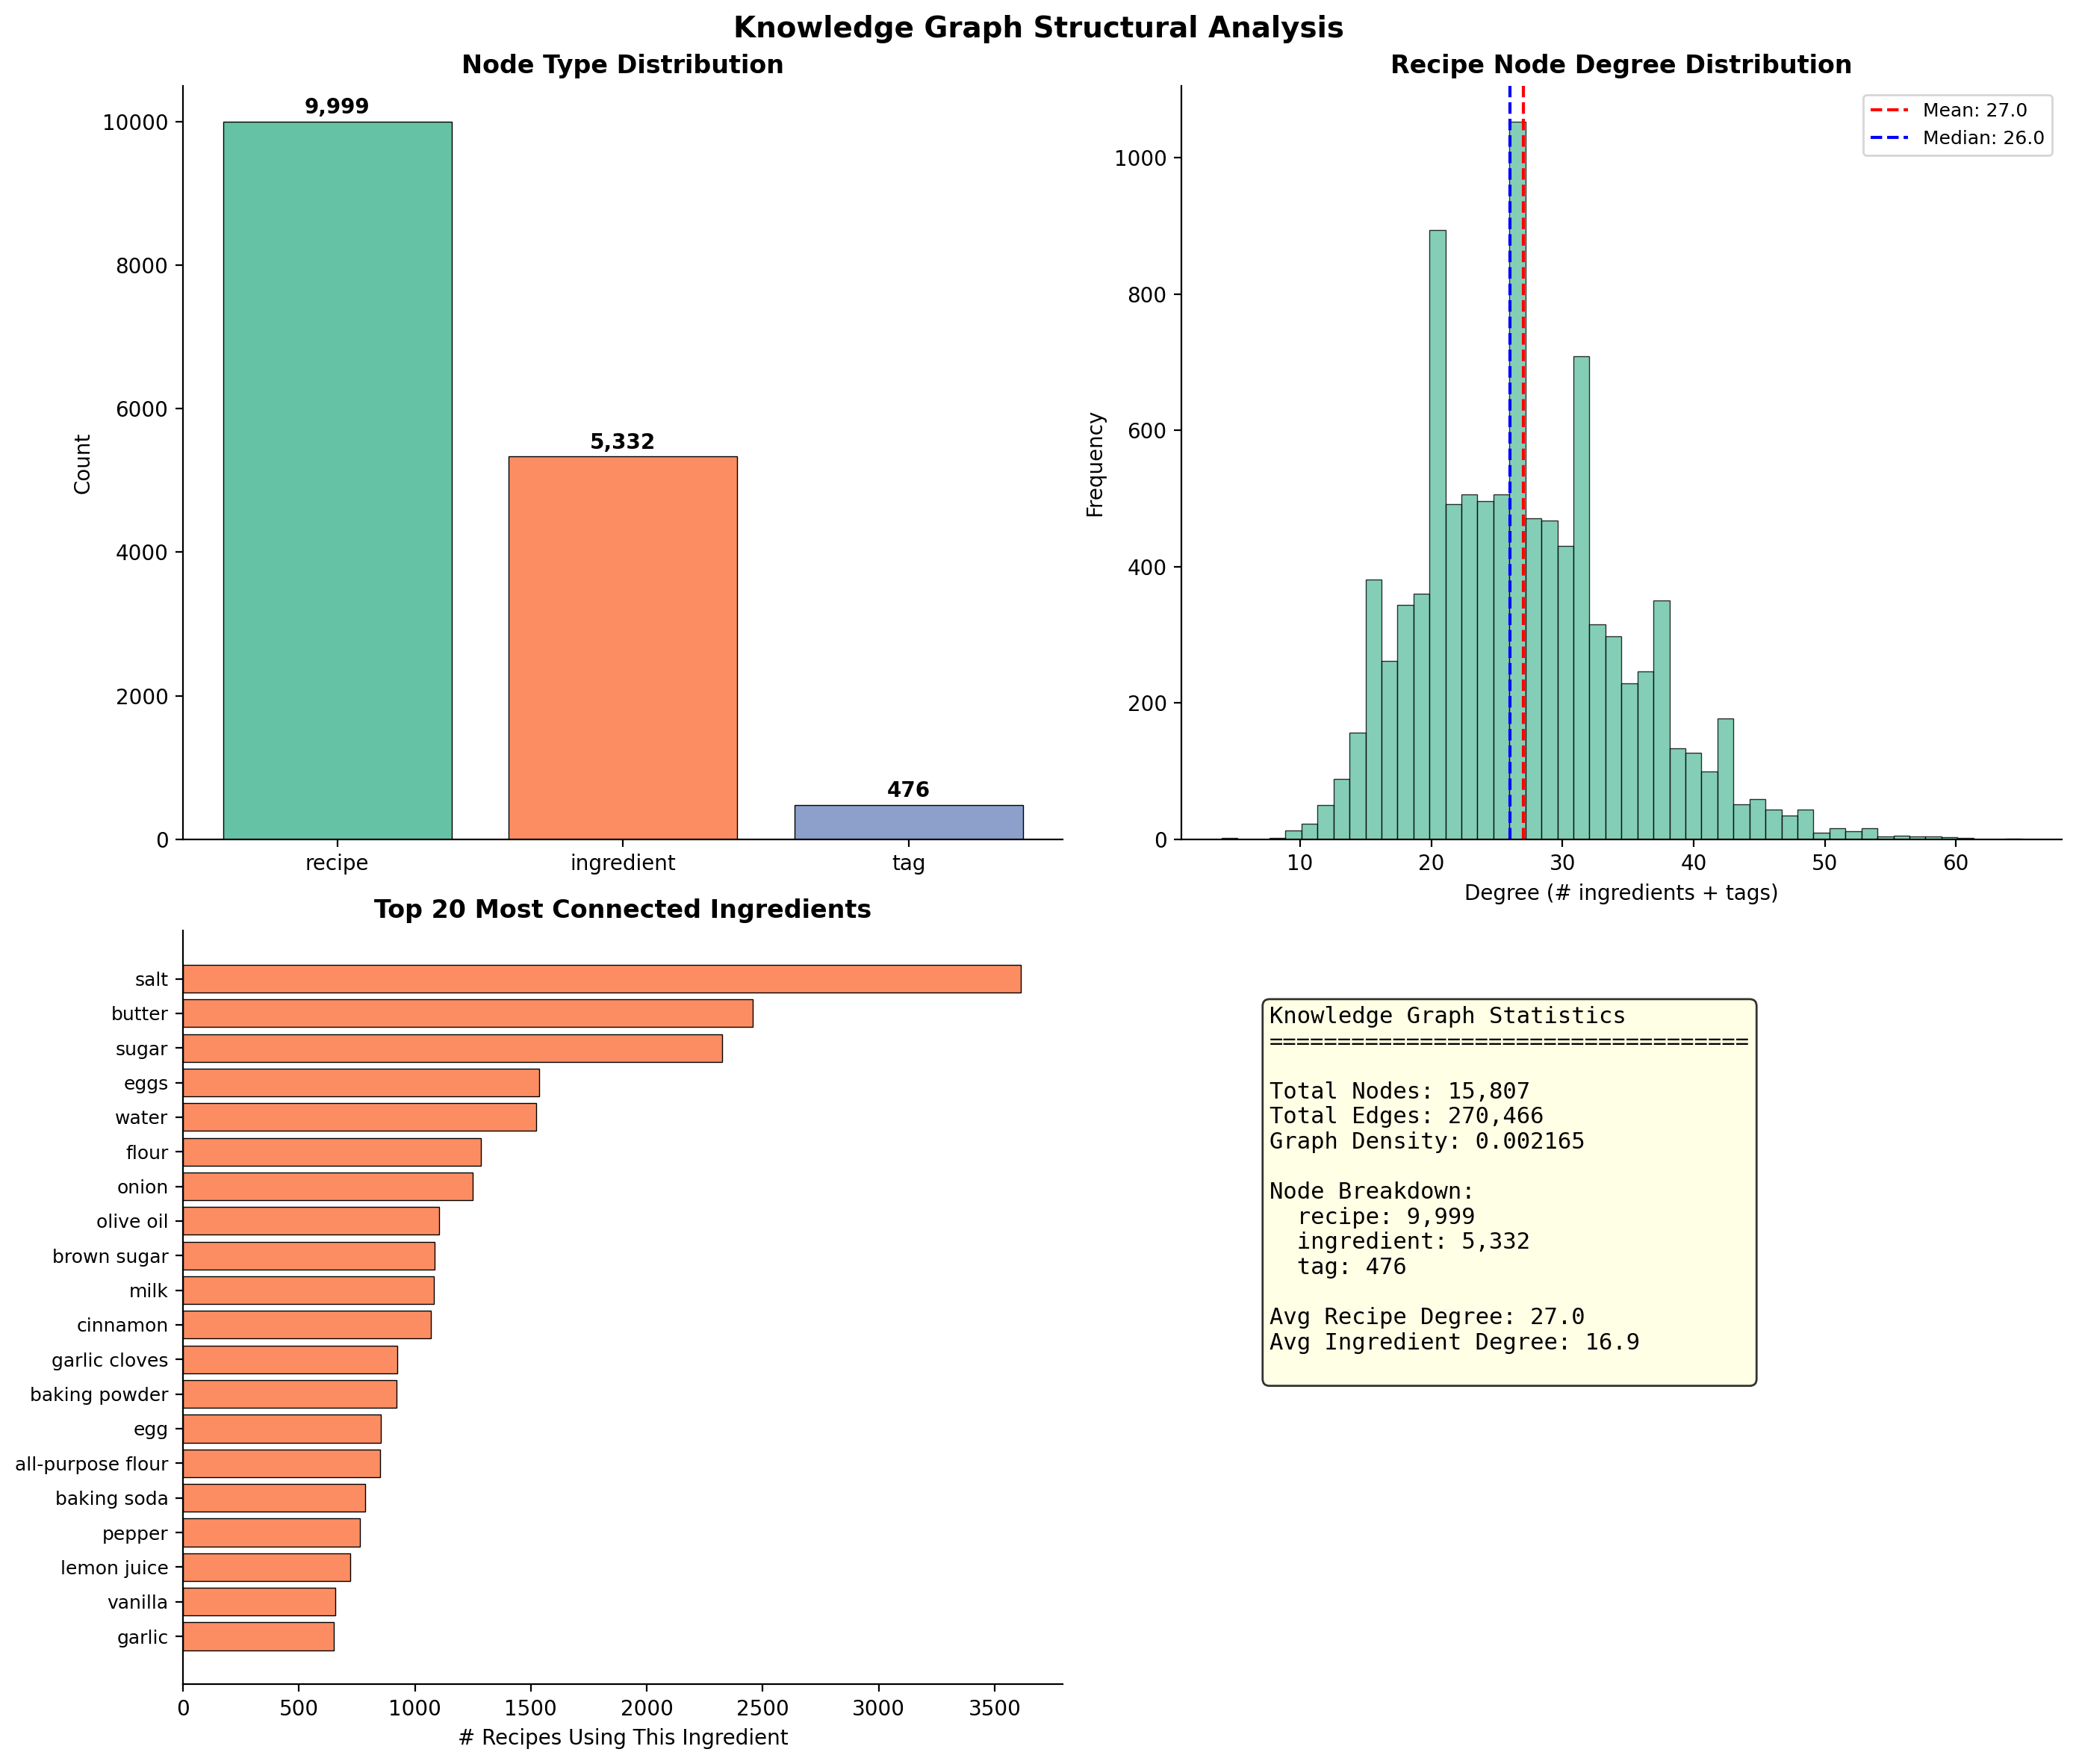
\includegraphics[width=\columnwidth]{kg_analysis.png}
\caption{Knowledge graph structural analysis: node type distribution, recipe degree distribution, and top connected ingredients.}
\label{fig:kg_analysis}
\end{figure}

\subsection{Stateful Memory System}

The memory system implements a write-summarize-retrieve pattern using SQLite:
\begin{itemize}[nosep]
    \item \textbf{Write:} After every pipeline run, the session's recipes and constraints are stored
    \item \textbf{Summarize:} Every 3rd session, the LLM generates a natural-language summary of user patterns (preferred cuisines, time tolerance, allergen history)
    \item \textbf{Retrieve:} Before planning, the system retrieves the user's summary, preferences, and recent recipes to inject as context into the planner prompt
\end{itemize}
Users can also provide explicit per-recipe feedback (like/dislike) which is persisted and incorporated into preference learning.

\subsection{Tool Suite}

The executor dispatches five tools:
\begin{enumerate}[nosep]
    \item \textbf{recipe\_search}: Hybrid RAG retrieval with allergy pre-filtering
    \item \textbf{allergy\_checker}: Two-layer check (local alias matching + Open Food Facts API)
    \item \textbf{nutrition}: Converts Food.com PDV values to absolute nutritional amounts
    \item \textbf{grocery\_list}: Aggregates and categorizes ingredients across recipes
    \item \textbf{budget\_estimator}: Estimates grocery cost using USDA/BLS average prices
\end{enumerate}

\subsection{Safety and Guardrails}

The system implements domain-appropriate safety measures:
\begin{itemize}[nosep]
    \item Blocked keyword filter for unsafe food requests
    \item Input length limits (2000 characters)
    \item Allergy verification at two levels (local + API)
    \item Critic-based retry on constraint violations
    \item Structured logging of all prompts, tool calls, and outputs
\end{itemize}

% ============================================================
\section{Dataset}

\subsection{Food.com Recipes}

The primary dataset is the Food.com Recipes and User Interactions dataset from Kaggle, containing 231,637 recipes. Each recipe includes: name, cooking time (minutes), tags (dietary, cuisine, cooking method), nutrition (7 PDV values), ingredient list, and preparation steps. After cleaning, 9,999 recipes are indexed for retrieval.

\subsection{Open Food Facts API}

The Open Food Facts database is queried at runtime to cross-check ingredient-level allergen labels, providing a second verification layer beyond local string matching.

\subsection{Evaluation Test Sets}

We created two evaluation sets:

\textbf{Structured Test Cases (60):} Each case specifies constraints (meal count, max cooking time, dietary tags, allergens) and expected outputs (minimum meals, time limits, forbidden allergens). These test end-to-end pipeline correctness.

\textbf{Dynamic Scenarios (205):} Generated programmatically across four complexity levels (simple: 70, medium: 70, complex: 60, edge cases: 5). Include natural language inputs and additional constraints like ingredients on hand and cuisine preferences.

\subsection{Retrieval Ground Truth}

For evaluating the retrieval pipeline independently, we generated ground truth relevance judgments from the dataset itself (no LLM calls, fully reproducible):
\begin{itemize}[nosep]
    \item \textbf{Tag-based queries} (150): Single-tag and paired-tag queries with known relevant recipe sets
    \item \textbf{Ingredient-based queries} (100): Single and multi-ingredient queries
    \item \textbf{KG-graded queries} (50): Graded relevance (0--3) based on ingredient overlap ratios ($\geq$60\%=3, 30--59\%=2, 10--29\%=1)
    \item \textbf{Natural language queries} (30): Realistic user queries combining ingredients, dietary preferences, and time constraints
\end{itemize}
Total: 330 queries with deterministic relevance judgments.

% ============================================================
\section{Multi-Model Comparison}

\subsection{Models Evaluated}

We compare four LLMs spanning cloud and local deployment:

\begin{table}[H]
\centering
\caption{Models evaluated in this study.}
\label{tab:models}
\small
\begin{tabular}{@{}llll@{}}
\toprule
\textbf{Model} & \textbf{Provider} & \textbf{Type} & \textbf{Params} \\
\midrule
Llama 3.3 70B & Groq & Open & 70B \\
Llama 3.2 3B & Ollama & Open & 3B \\
Granite 3.1 2B & Ollama & Open & 2B \\
Gemini 2.5 Flash Lite & Google & Closed & -- \\
\bottomrule
\end{tabular}
\end{table}

All models are evaluated on the same 60-case test set. Gemini evaluation was limited by the free-tier daily API quota (requests per day), so we report results for the three models with complete evaluations.

\subsection{End-to-End Pipeline Results}

Table~\ref{tab:pipeline_results} summarizes performance across all models. All three models achieve 100\% constraint pass rate, demonstrating that the Planner-Executor-Critic architecture reliably produces valid meal plans regardless of the underlying LLM.

\begin{table}[H]
\centering
\caption{End-to-end pipeline evaluation results (60-case test set).}
\label{tab:pipeline_results}
\small
\begin{tabular}{@{}lccc@{}}
\toprule
\textbf{Metric} & \textbf{Llama 70B} & \textbf{Llama 3B} & \textbf{Granite 2B} \\
 & \textbf{(Groq)} & \textbf{(Ollama)} & \textbf{(Ollama)} \\
\midrule
Cases Completed & 23/60 & 60/60 & 60/60 \\
Constraint Pass & 100\% & 100\% & 100\% \\
Allergy Violation & 0.0\% & 0.9\% & 1.0\% \\
Citation Pass & 100\% & 100\% & 100\% \\
Tool Success & 100\% & 100\% & 100\% \\
Critic Valid & 100\% & 96.7\% & 95.0\% \\
Avg Retries & 0.09 & 0.20 & 0.15 \\
Avg Latency & 12.8s & 30.9s & 25.9s \\
\bottomrule
\end{tabular}
\end{table}

Key findings:
\begin{itemize}[nosep]
    \item \textbf{Llama 3.3 70B (Groq):} Highest quality (0\% allergy violations, 100\% critic validity) and fastest (12.8s) due to Groq's hardware acceleration. Only 23/60 cases completed due to free-tier rate limits.
    \item \textbf{Llama 3.2 3B:} Complete evaluation with strong results. Minor allergy violations (0.9\%) from edge cases where ingredient names are ambiguous. Higher retry rate (0.20) suggests the smaller model occasionally produces malformed plans.
    \item \textbf{Granite 3.1 2B:} Comparable quality to Llama 3B despite being 33\% smaller. Slightly higher allergy violation rate (1.0\%) and lower critic validity (95\%).
\end{itemize}

\subsection{Cost and Latency Tradeoffs}

\begin{figure}[H]
\centering
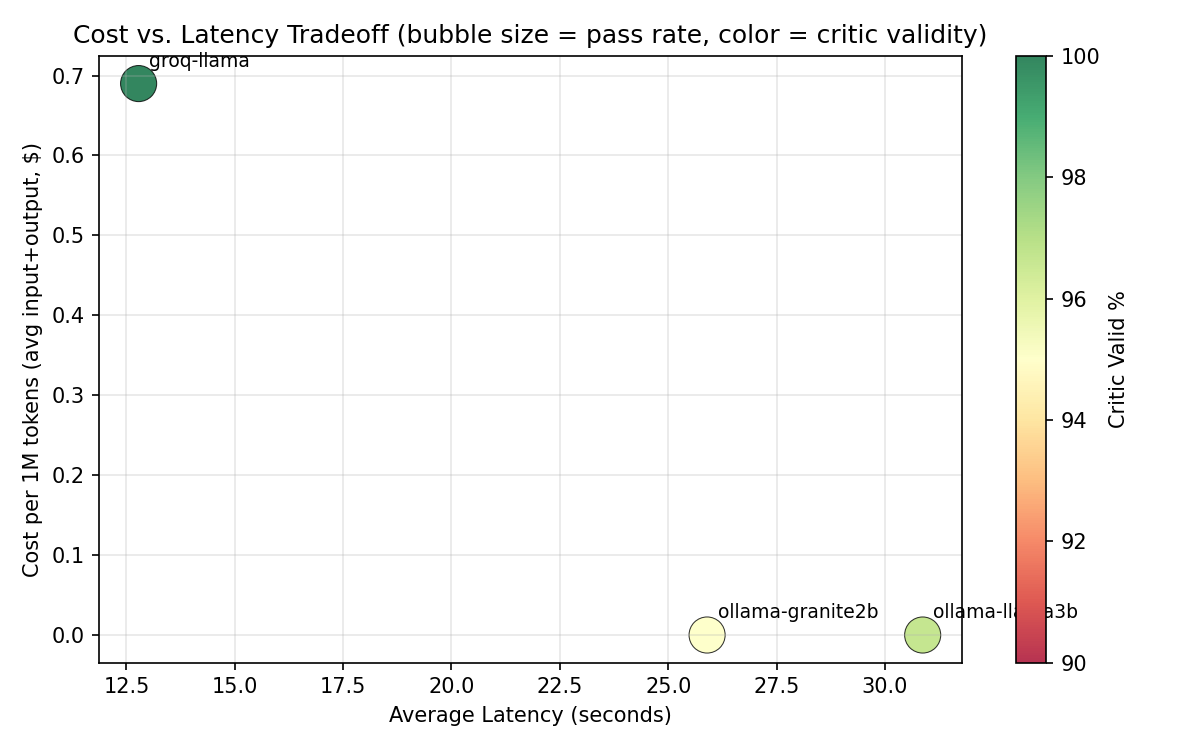
\includegraphics[width=\columnwidth]{cost_latency_scatter.png}
\caption{Cost vs.\ latency tradeoff. Bubble size indicates constraint pass rate, color indicates critic validity rate.}
\label{fig:cost_latency}
\end{figure}

Figure~\ref{fig:cost_latency} shows the cost-latency tradeoff. Groq offers the best latency (12.8s) at \$0.69/1M tokens. The local Ollama models run at zero cost but 2--2.5$\times$ higher latency. For production deployment, Groq provides the best quality-latency balance; for offline or privacy-sensitive applications, Ollama models are viable alternatives.

\begin{figure}[H]
\centering
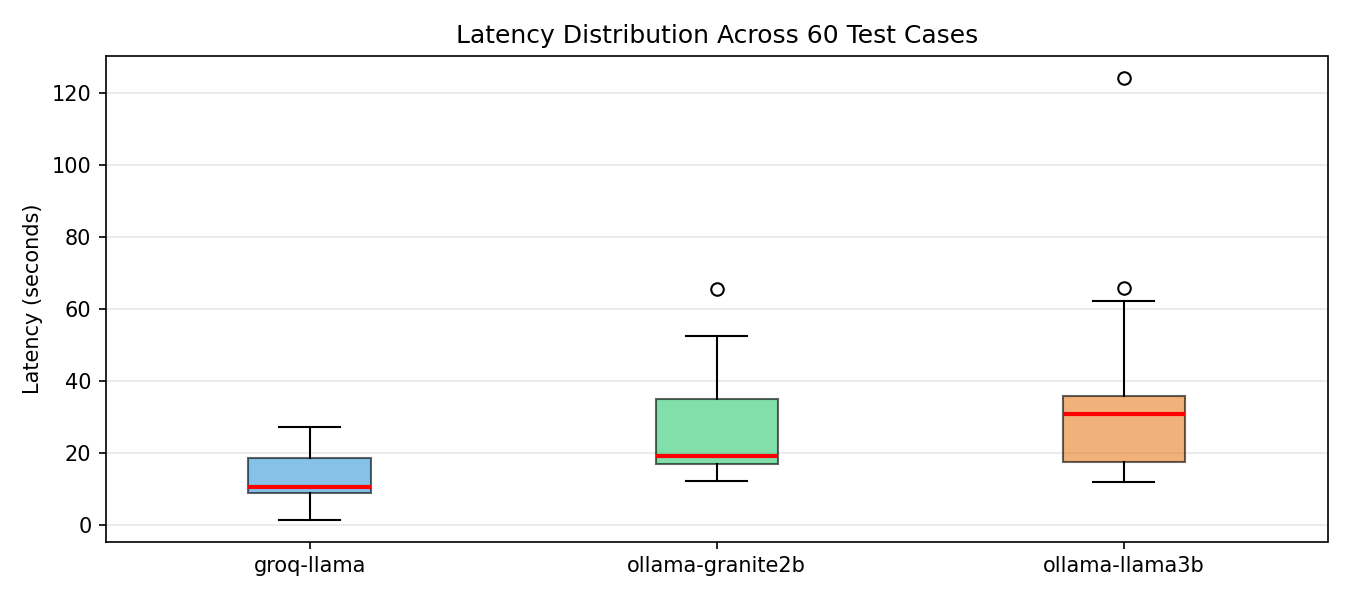
\includegraphics[width=\columnwidth]{latency_distribution.png}
\caption{Latency distribution across 60 test cases per model. Groq shows the tightest distribution due to dedicated inference hardware.}
\label{fig:latency_dist}
\end{figure}

\begin{figure}[H]
\centering
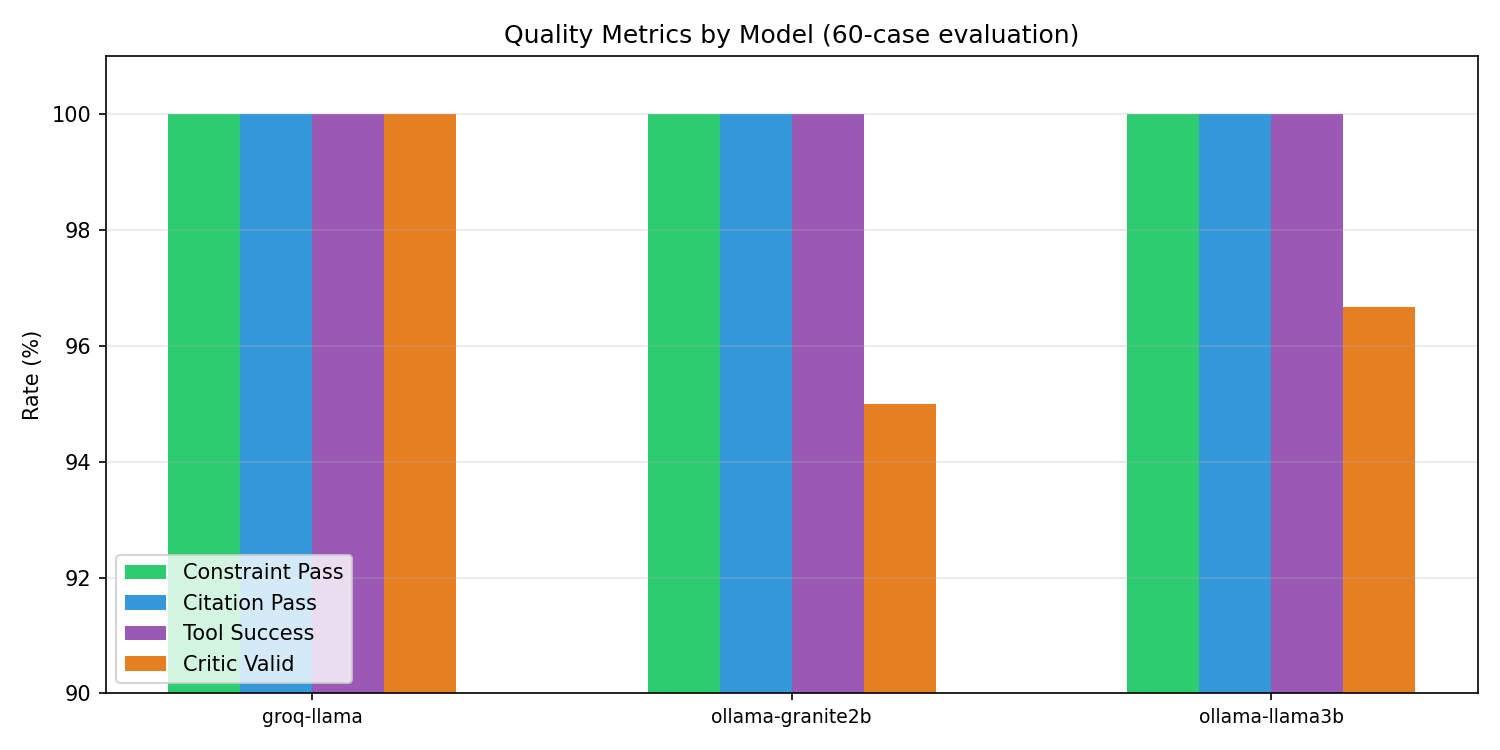
\includegraphics[width=\columnwidth]{quality_metrics.png}
\caption{Quality metrics comparison across models. All models achieve $\geq$95\% on all metrics.}
\label{fig:quality_metrics}
\end{figure}

\begin{figure}[H]
\centering
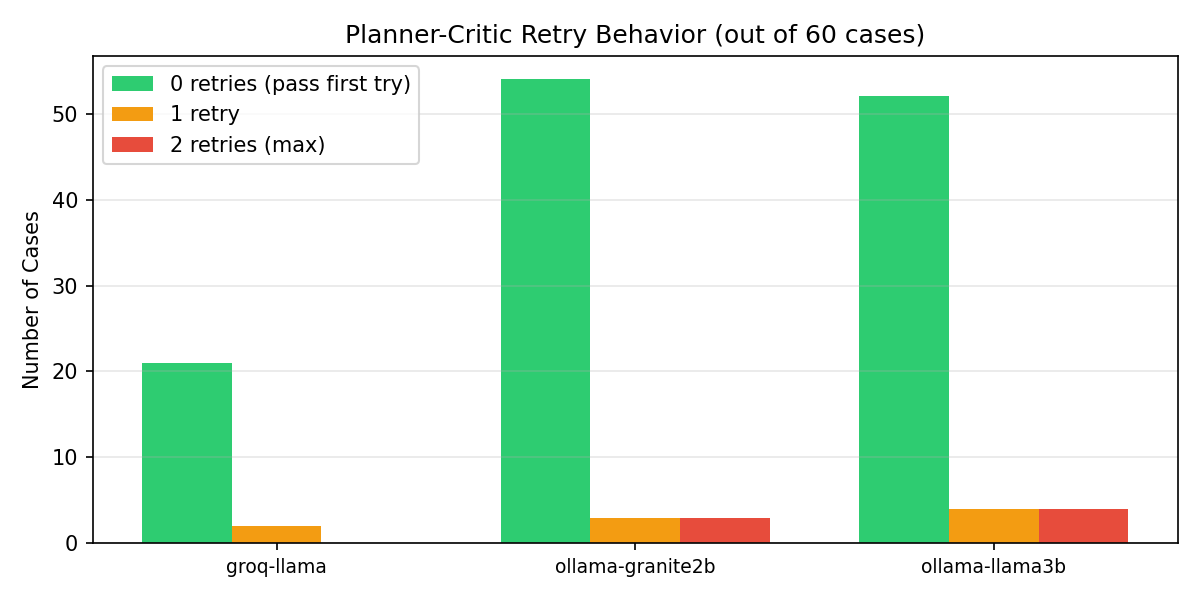
\includegraphics[width=\columnwidth]{retry_behavior.png}
\caption{Planner-Critic retry behavior. Most cases pass on the first attempt. Smaller models require more retries.}
\label{fig:retry_behavior}
\end{figure}

% ============================================================
\section{Retrieval Evaluation}

\subsection{Methodology}

We evaluate retrieval quality independently from the end-to-end pipeline using standard IR metrics:
\begin{itemize}[nosep]
    \item \textbf{Precision@k}: Fraction of top-$k$ results that are relevant
    \item \textbf{Recall@k}: Fraction of all relevant documents found in top-$k$
    \item \textbf{MRR}: Reciprocal rank of the first relevant result
    \item \textbf{NDCG@k}: Normalized discounted cumulative gain (graded relevance)
    \item \textbf{MAP}: Mean average precision across queries
\end{itemize}

\subsection{Ablation Study}

We systematically disable retrieval components to measure their individual and combined contributions. Table~\ref{tab:ablation} shows results across 6 configurations.

\begin{table}[H]
\centering
\caption{Retrieval ablation study results (330 ground truth queries).}
\label{tab:ablation}
\small
\begin{tabular}{@{}lccccc@{}}
\toprule
\textbf{Config} & \textbf{P@5} & \textbf{P@10} & \textbf{R@10} & \textbf{MRR} & \textbf{NDCG} \\
\midrule
Vector only & .255 & .233 & .075 & .373 & .154 \\
BM25 only & .575 & .535 & .314 & .648 & .361 \\
Vector+BM25 & .365 & .415 & .241 & .502 & .234 \\
Vector+KG & .365 & .308 & .092 & .466 & .189 \\
BM25+KG & .580 & .550 & .323 & .673 & .370 \\
\textbf{Full hybrid} & \textbf{.655} & \textbf{.568} & \textbf{.338} & \textbf{.688} & \textbf{.438} \\
\bottomrule
\end{tabular}
\end{table}

\begin{figure}[H]
\centering
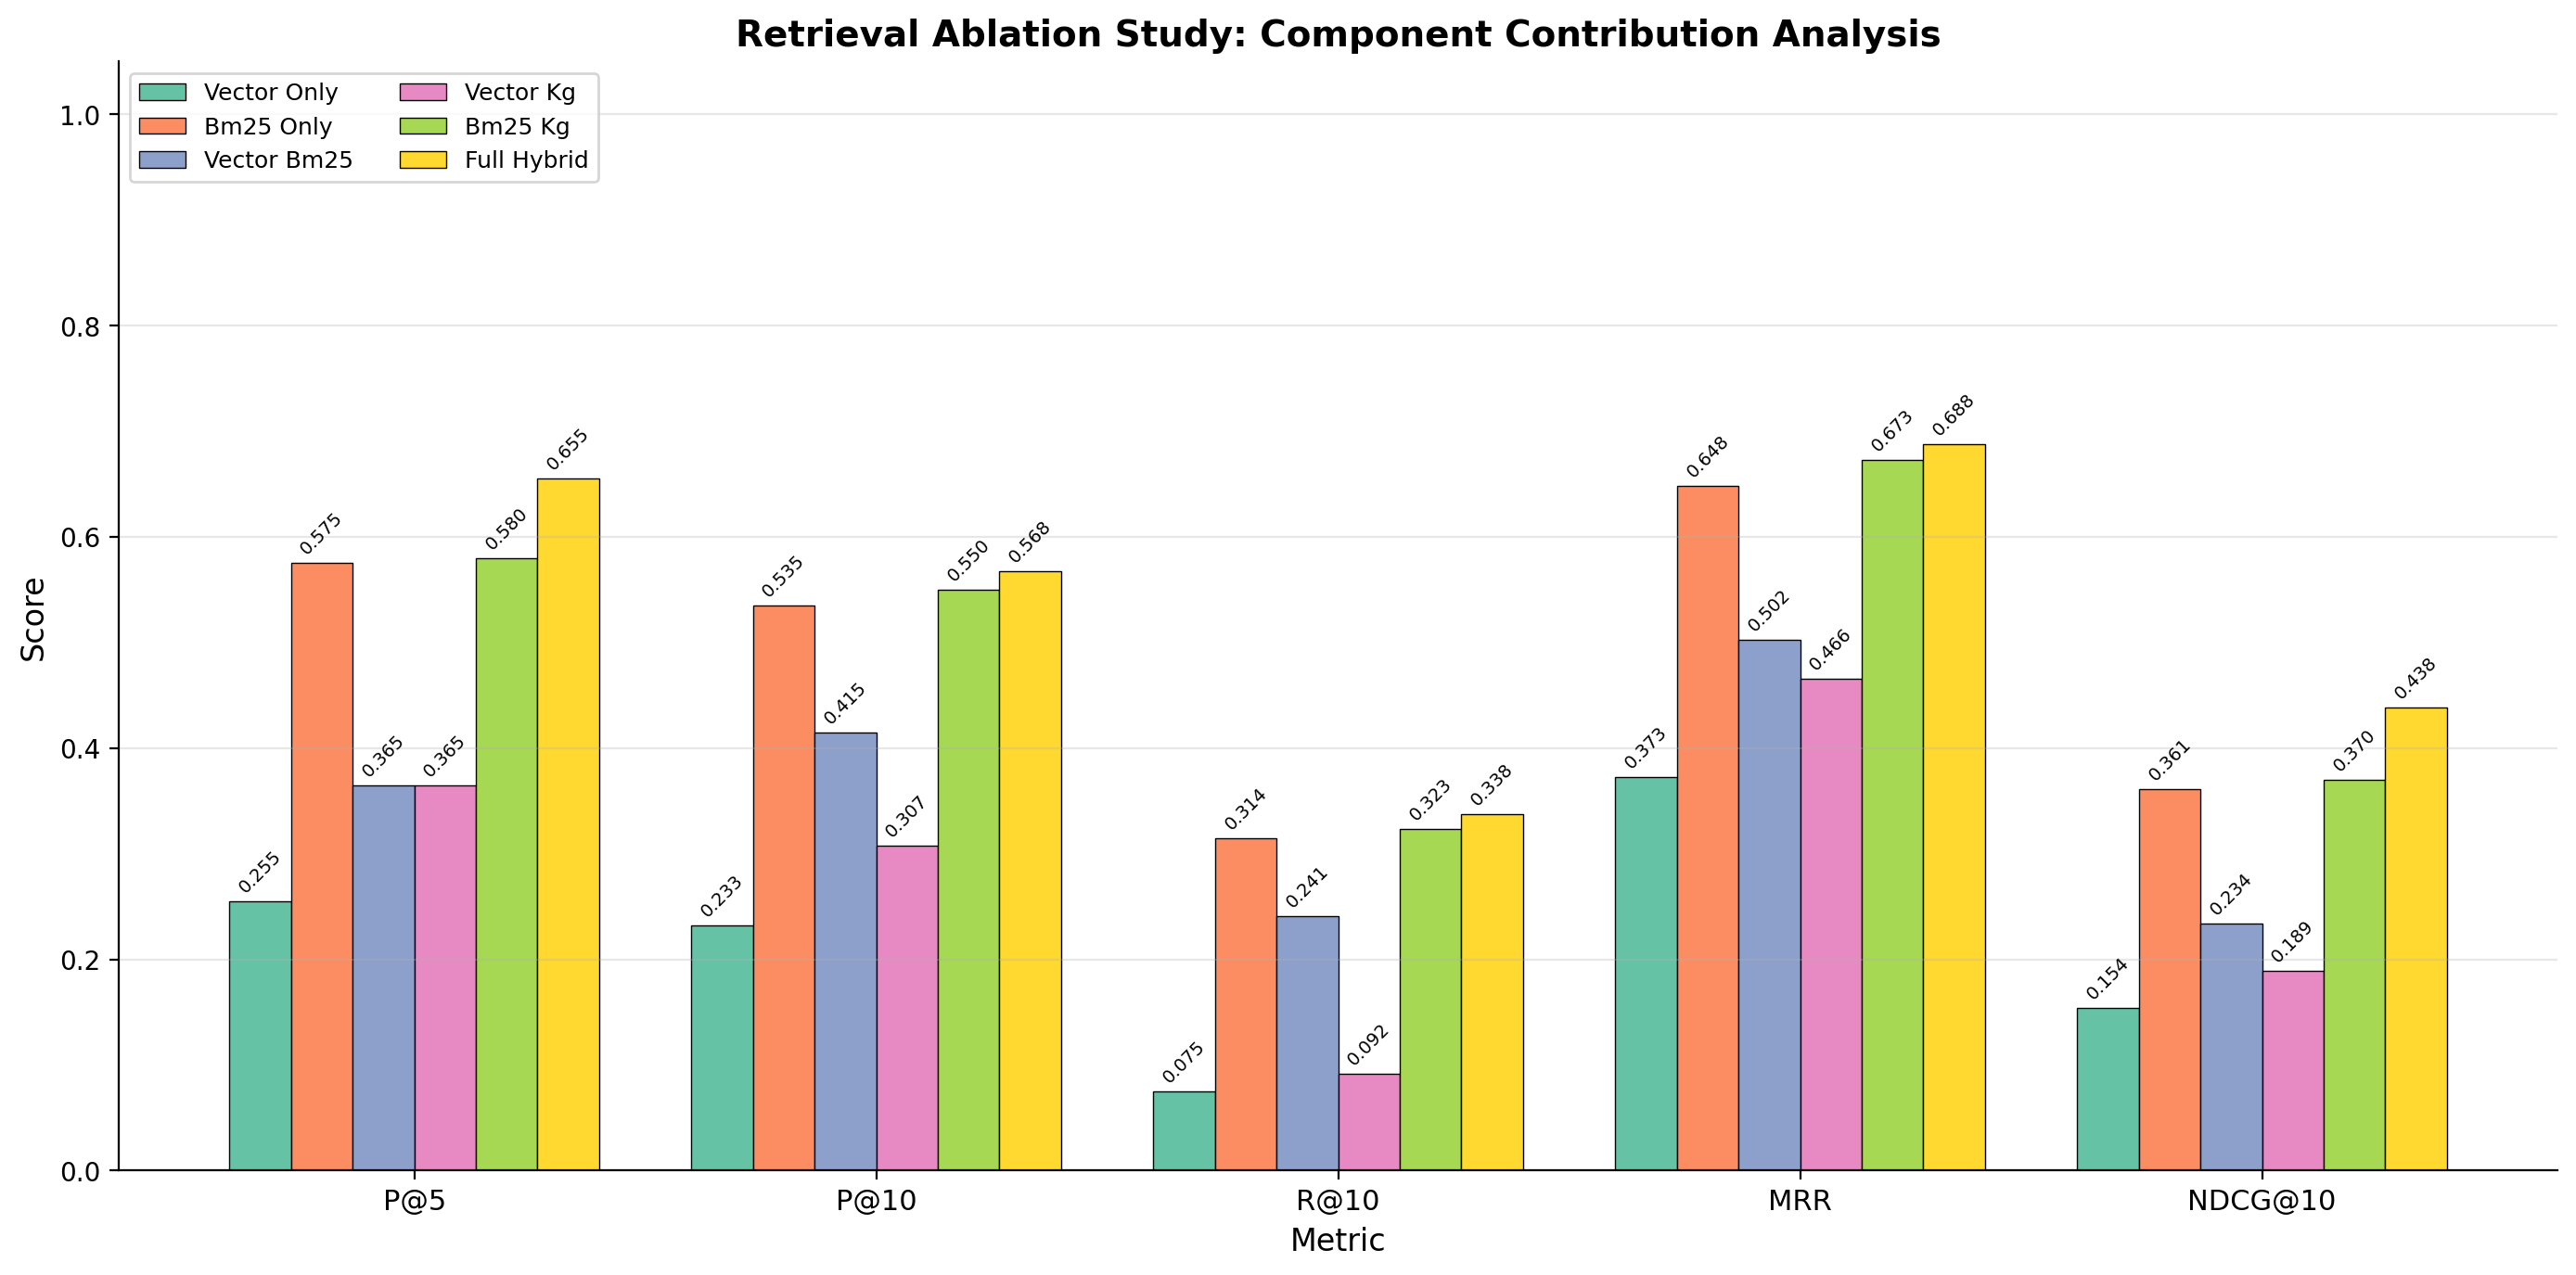
\includegraphics[width=\columnwidth]{ablation_comparison.png}
\caption{Ablation study: grouped bar chart comparing all retrieval configurations across key metrics. Full hybrid consistently achieves the highest scores.}
\label{fig:ablation}
\end{figure}

Key findings from the ablation:
\begin{itemize}[nosep]
    \item \textbf{BM25 dominates vector retrieval} for this domain. Recipe text contains highly specific ingredient and tag keywords that BM25 matches effectively. Dense embeddings capture semantic similarity but rank lower on exact-match queries.
    \item \textbf{KG re-ranking consistently improves BM25}: BM25+KG outperforms BM25 alone on every metric (e.g., MRR: 0.648 $\rightarrow$ 0.673).
    \item \textbf{Full hybrid achieves the best results}: Combining all three components yields P@5=0.655, which is 14\% above BM25 alone and 157\% above vector alone.
    \item \textbf{RRF fusion underperforms when vector quality is low}: Vector+BM25 (0.502 MRR) is lower than BM25 alone (0.648), because noisy vector results dilute the BM25 signal. The KG's preference-aware boost corrects this in the full hybrid.
\end{itemize}

\begin{figure}[H]
\centering
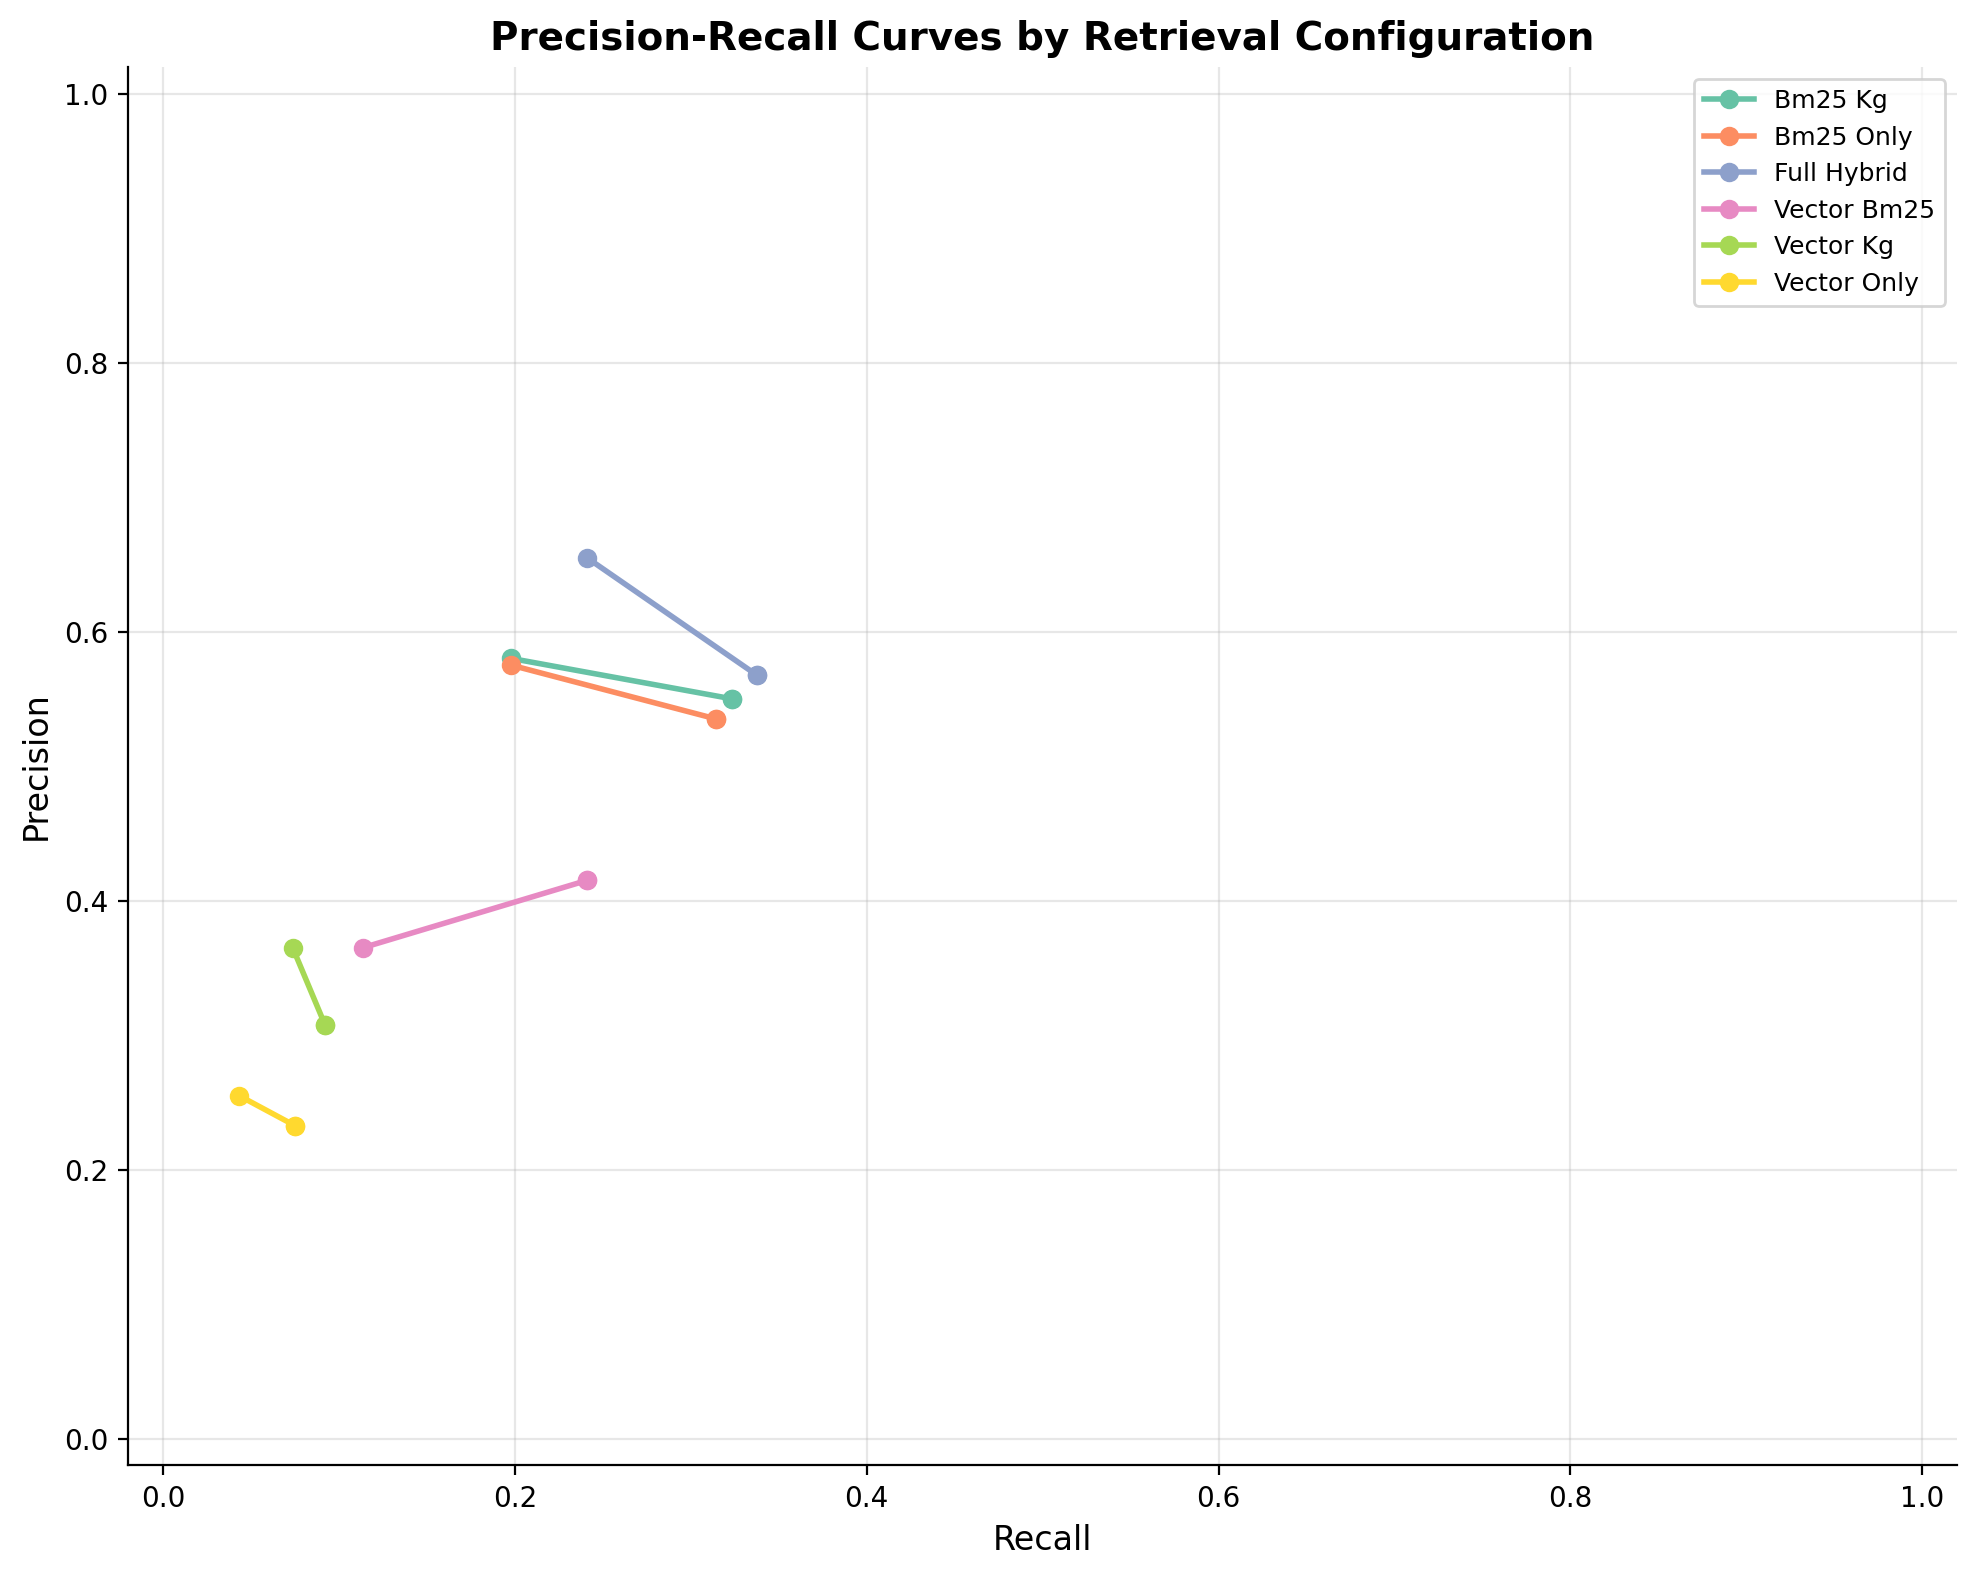
\includegraphics[width=\columnwidth]{precision_recall_curves.png}
\caption{Precision-recall curves as $k$ varies. Full hybrid maintains the best precision at all recall levels.}
\label{fig:pr_curves}
\end{figure}

\begin{figure}[H]
\centering
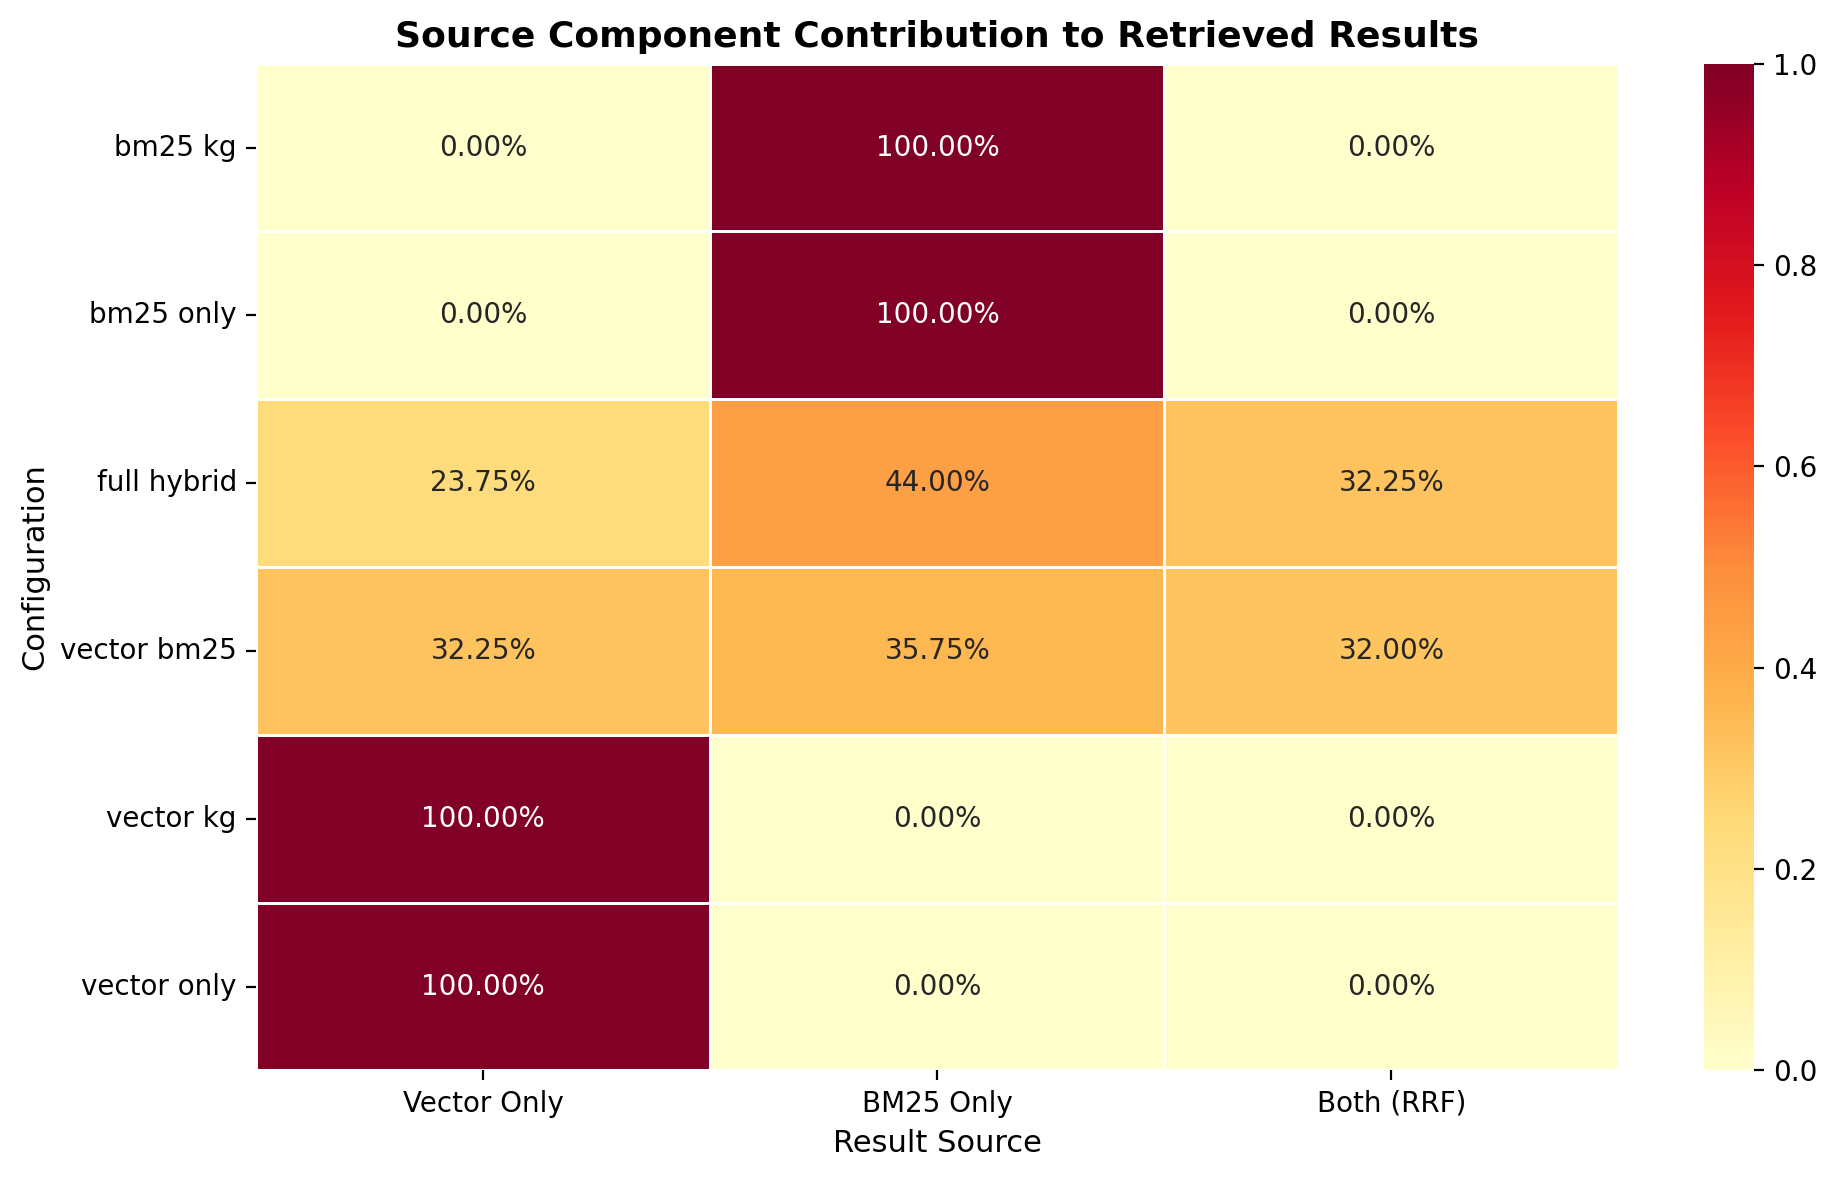
\includegraphics[width=\columnwidth]{component_contribution.png}
\caption{Source contribution heatmap: fraction of top-10 results from each retriever component. In the full hybrid, 44\% come from BM25, 24\% from vector, and 32\% from both (RRF overlap).}
\label{fig:component}
\end{figure}

\subsection{Performance by Query Type}

Figure~\ref{fig:query_type} breaks down MRR by query type. Tag-based queries (single and pair) achieve near-perfect MRR ($>$0.87) across all configurations. Ingredient queries show more differentiation, with BM25-based configs outperforming vector-only. Natural language queries and KG-graded queries are the most challenging, where the full hybrid's advantage is most pronounced.

\begin{figure}[H]
\centering
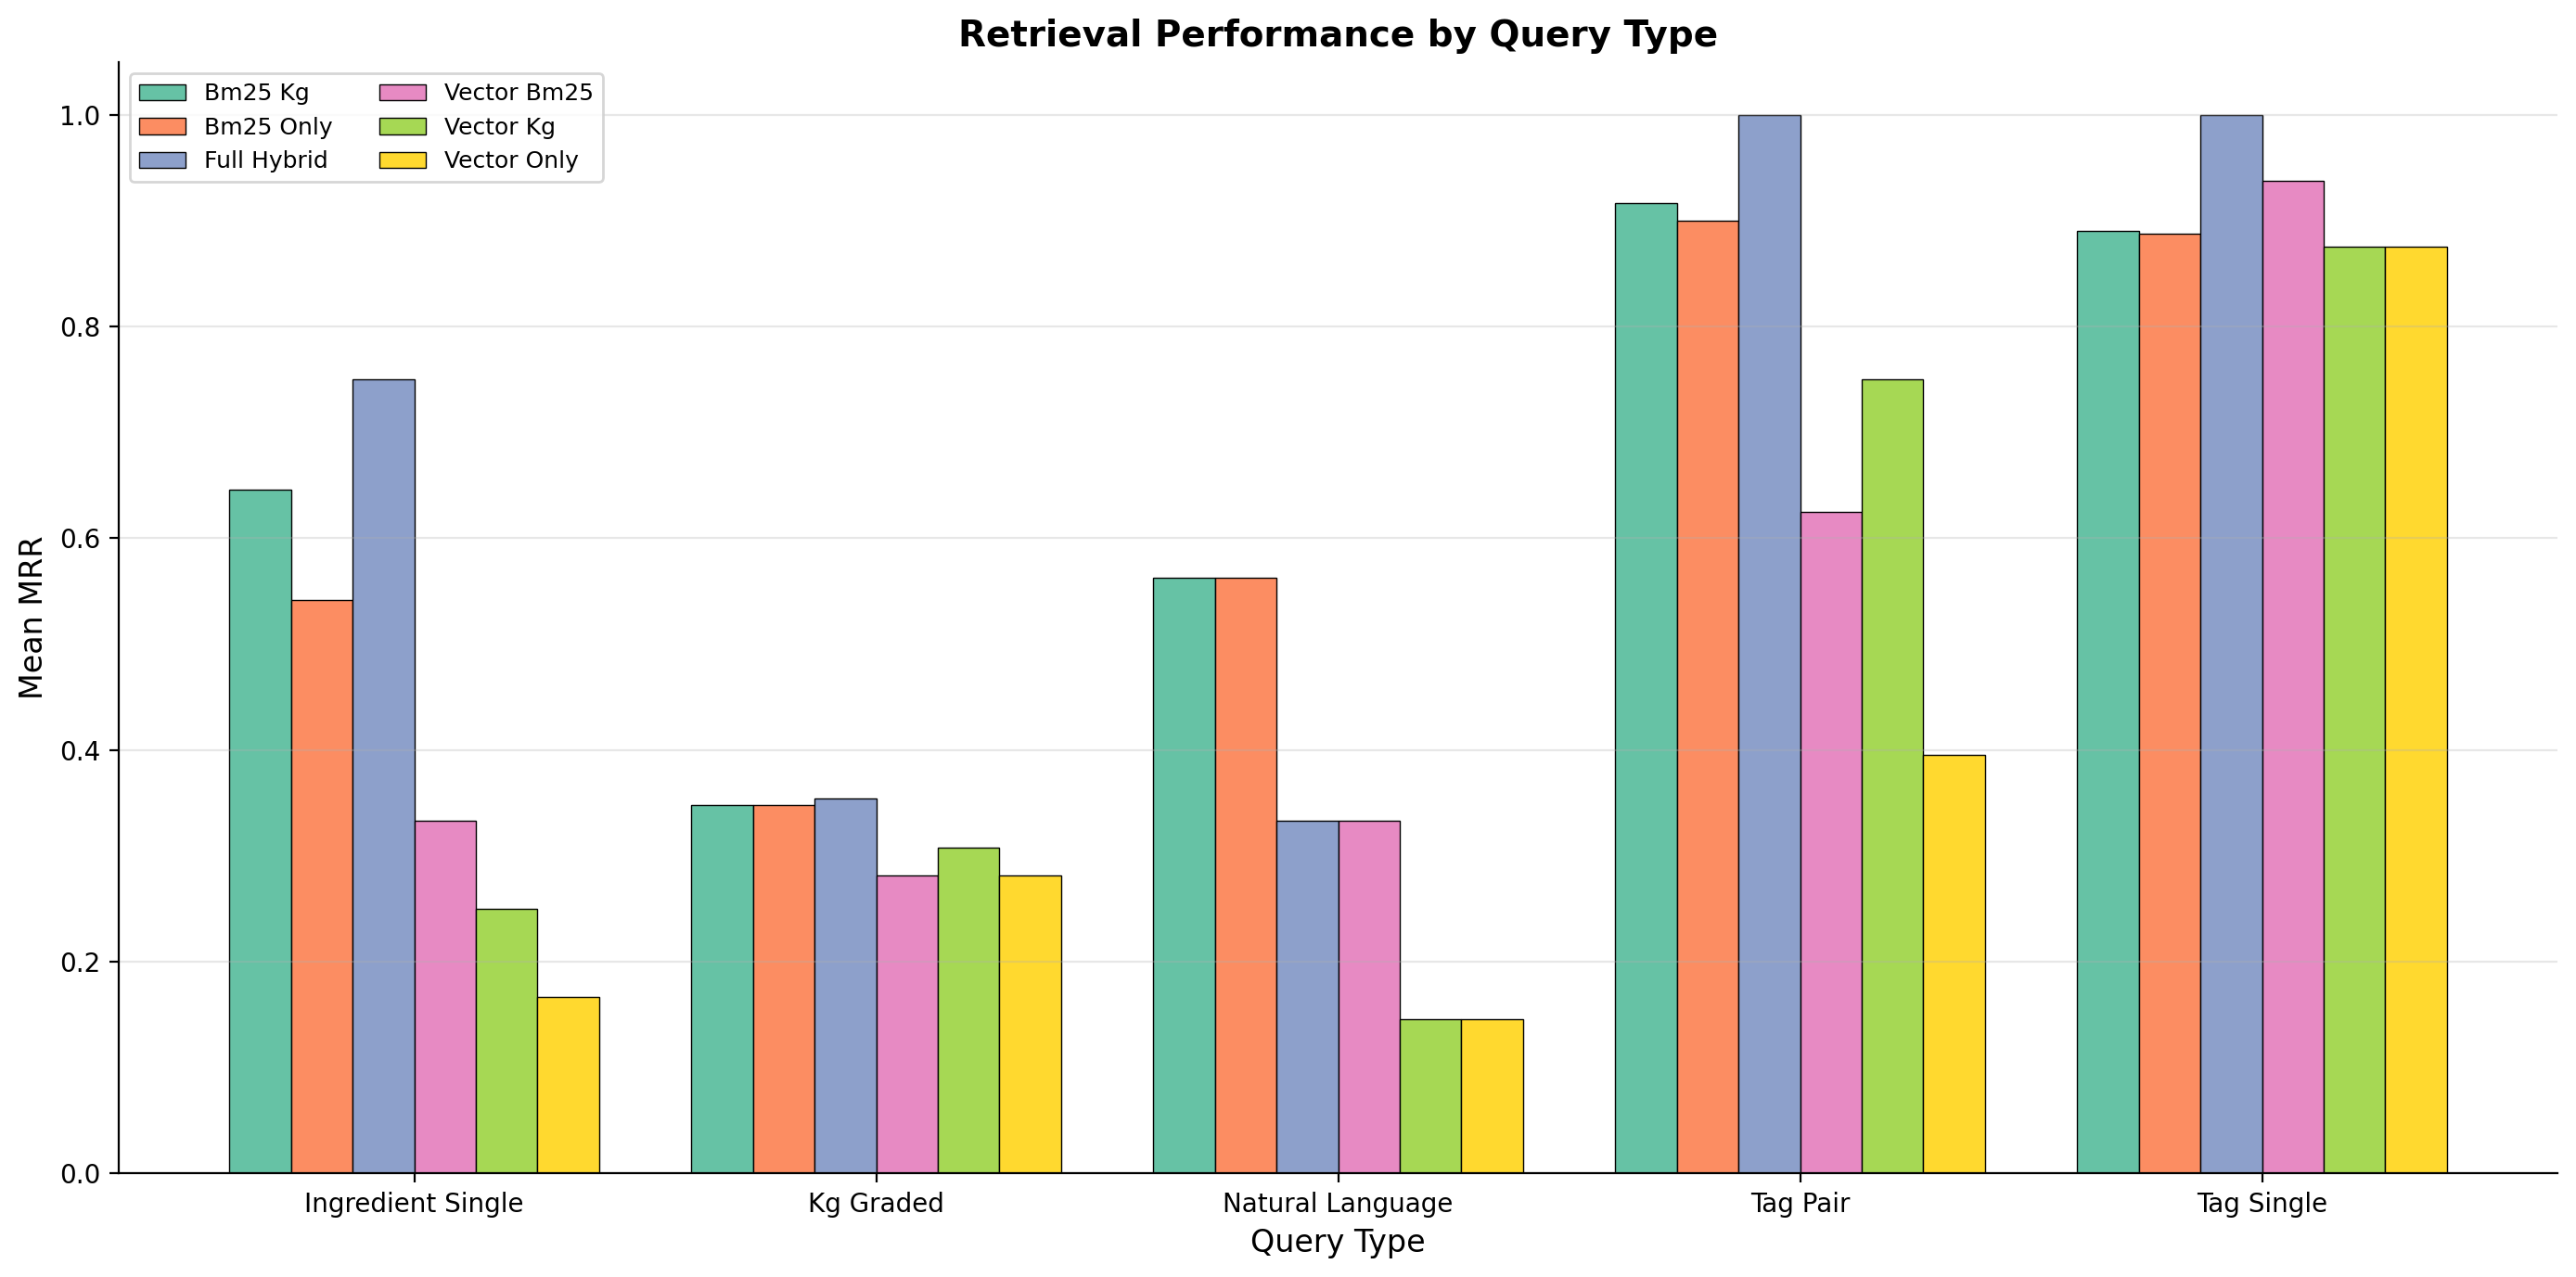
\includegraphics[width=\columnwidth]{query_type_breakdown.png}
\caption{Retrieval performance (MRR) broken down by query type. BM25-based configs excel on tag queries; the full hybrid has the largest advantage on complex query types.}
\label{fig:query_type}
\end{figure}

\subsection{Hyperparameter Sensitivity}

We sweep three key hyperparameters while holding others at defaults:

\textbf{Retrieval Depth (top\_k):} Performance improves from $k$=5 to $k$=20, then plateaus. MRR increases from 0.58 to 0.70. Recall continues increasing but precision drops, as expected.

\textbf{RRF Constant ($k$):} Relatively insensitive. MRR stays between 0.68--0.70 across $k \in \{10, 30, 60, 100, 200\}$. The default $k$=60 provides good balance.

\textbf{KG Boost Weight ($w$):} Small positive boost ($w$=0.05--0.1) improves MRR. Larger values ($w \geq 0.5$) cause over-reliance on graph structure. Optimal at $w$=0.1.

\begin{figure}[H]
\centering
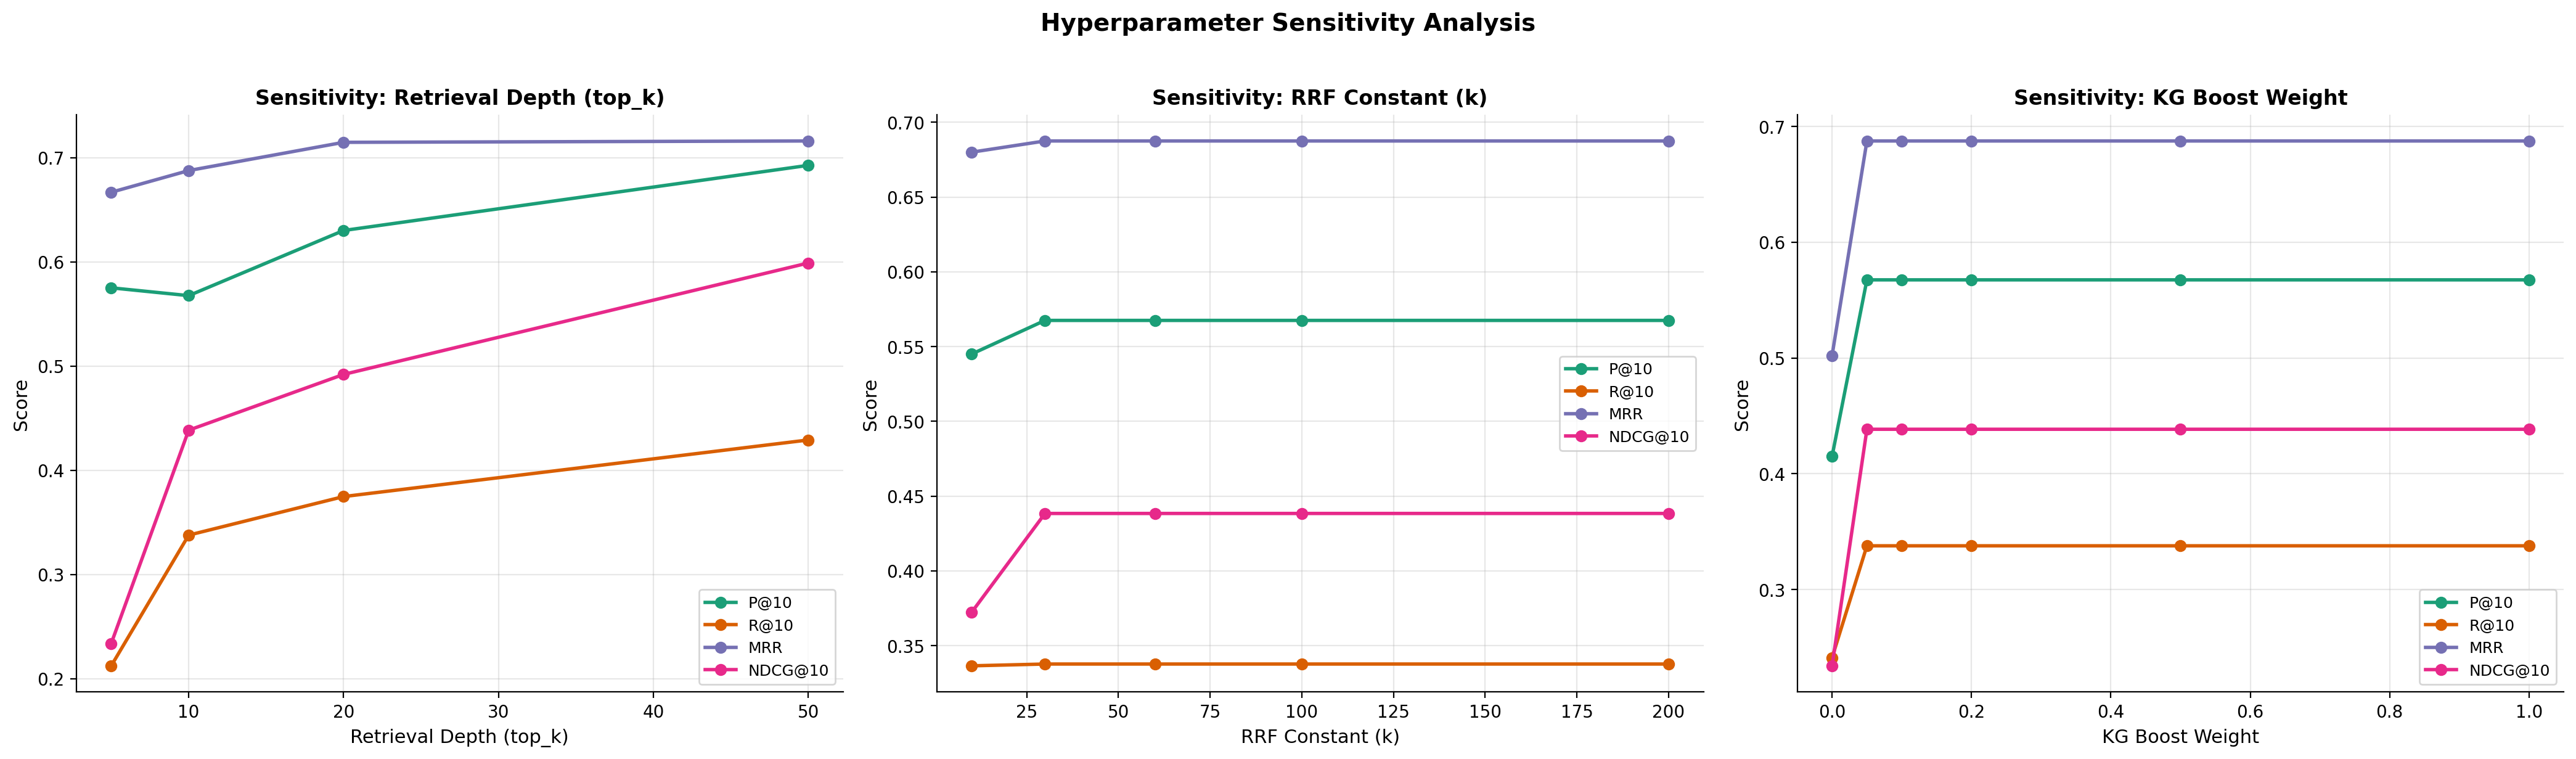
\includegraphics[width=\columnwidth]{hyperparam_sensitivity.png}
\caption{Hyperparameter sensitivity analysis. Three sweeps show the effect of top\_k, RRF constant, and KG boost weight on retrieval quality.}
\label{fig:hyperparam}
\end{figure}

\subsection{Statistical Significance}

We apply rigorous statistical testing to validate that performance differences between configurations are not due to chance:

\begin{itemize}[nosep]
    \item \textbf{Paired $t$-test}: Tests whether mean per-query metric differences are significant ($\alpha$=0.05)
    \item \textbf{Wilcoxon signed-rank test}: Non-parametric alternative, robust to non-normal score distributions
    \item \textbf{Bootstrap 95\% confidence intervals}: 1,000 bootstrap resamples per configuration
    \item \textbf{Cohen's $d$ effect size}: Quantifies practical significance ($|d|>$0.8 = large effect)
    \item \textbf{Bonferroni correction}: Adjusts $p$-values for multiple pairwise comparisons
\end{itemize}

\begin{figure}[H]
\centering
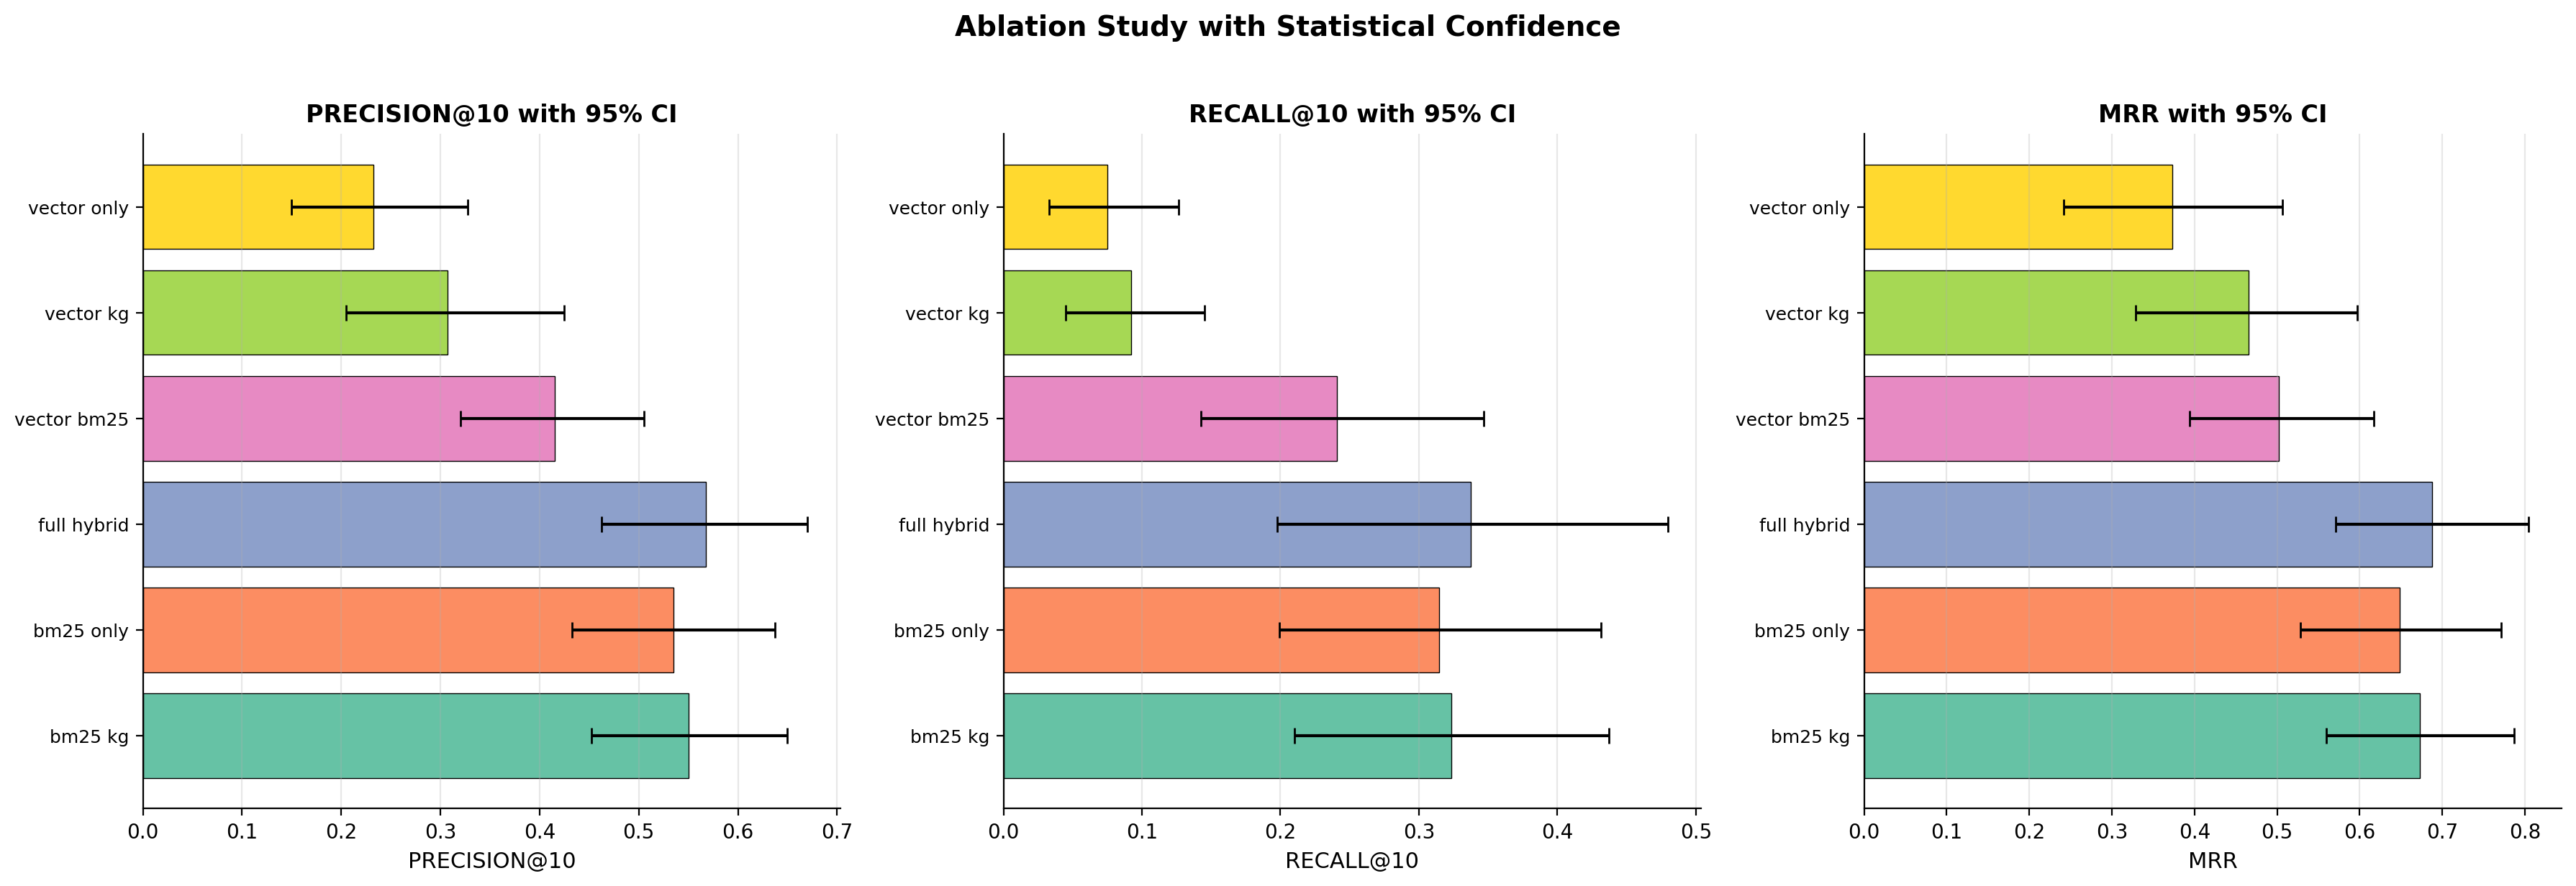
\includegraphics[width=\columnwidth]{ablation_with_ci.png}
\caption{Ablation results with bootstrap 95\% confidence intervals. Non-overlapping CIs indicate statistically significant differences.}
\label{fig:ablation_ci}
\end{figure}

Figure~\ref{fig:ablation_ci} shows the ablation results with confidence intervals. The full hybrid's precision@10 CI does not overlap with vector-only, confirming a statistically significant improvement. BM25-based configurations cluster together, with the full hybrid consistently at the top.

\subsection{Embedding Space Analysis}

Figure~\ref{fig:embedding} visualizes the recipe embedding space using t-SNE and UMAP projections of 2,000 recipe embeddings, colored by cuisine tag.

\begin{figure}[H]
\centering
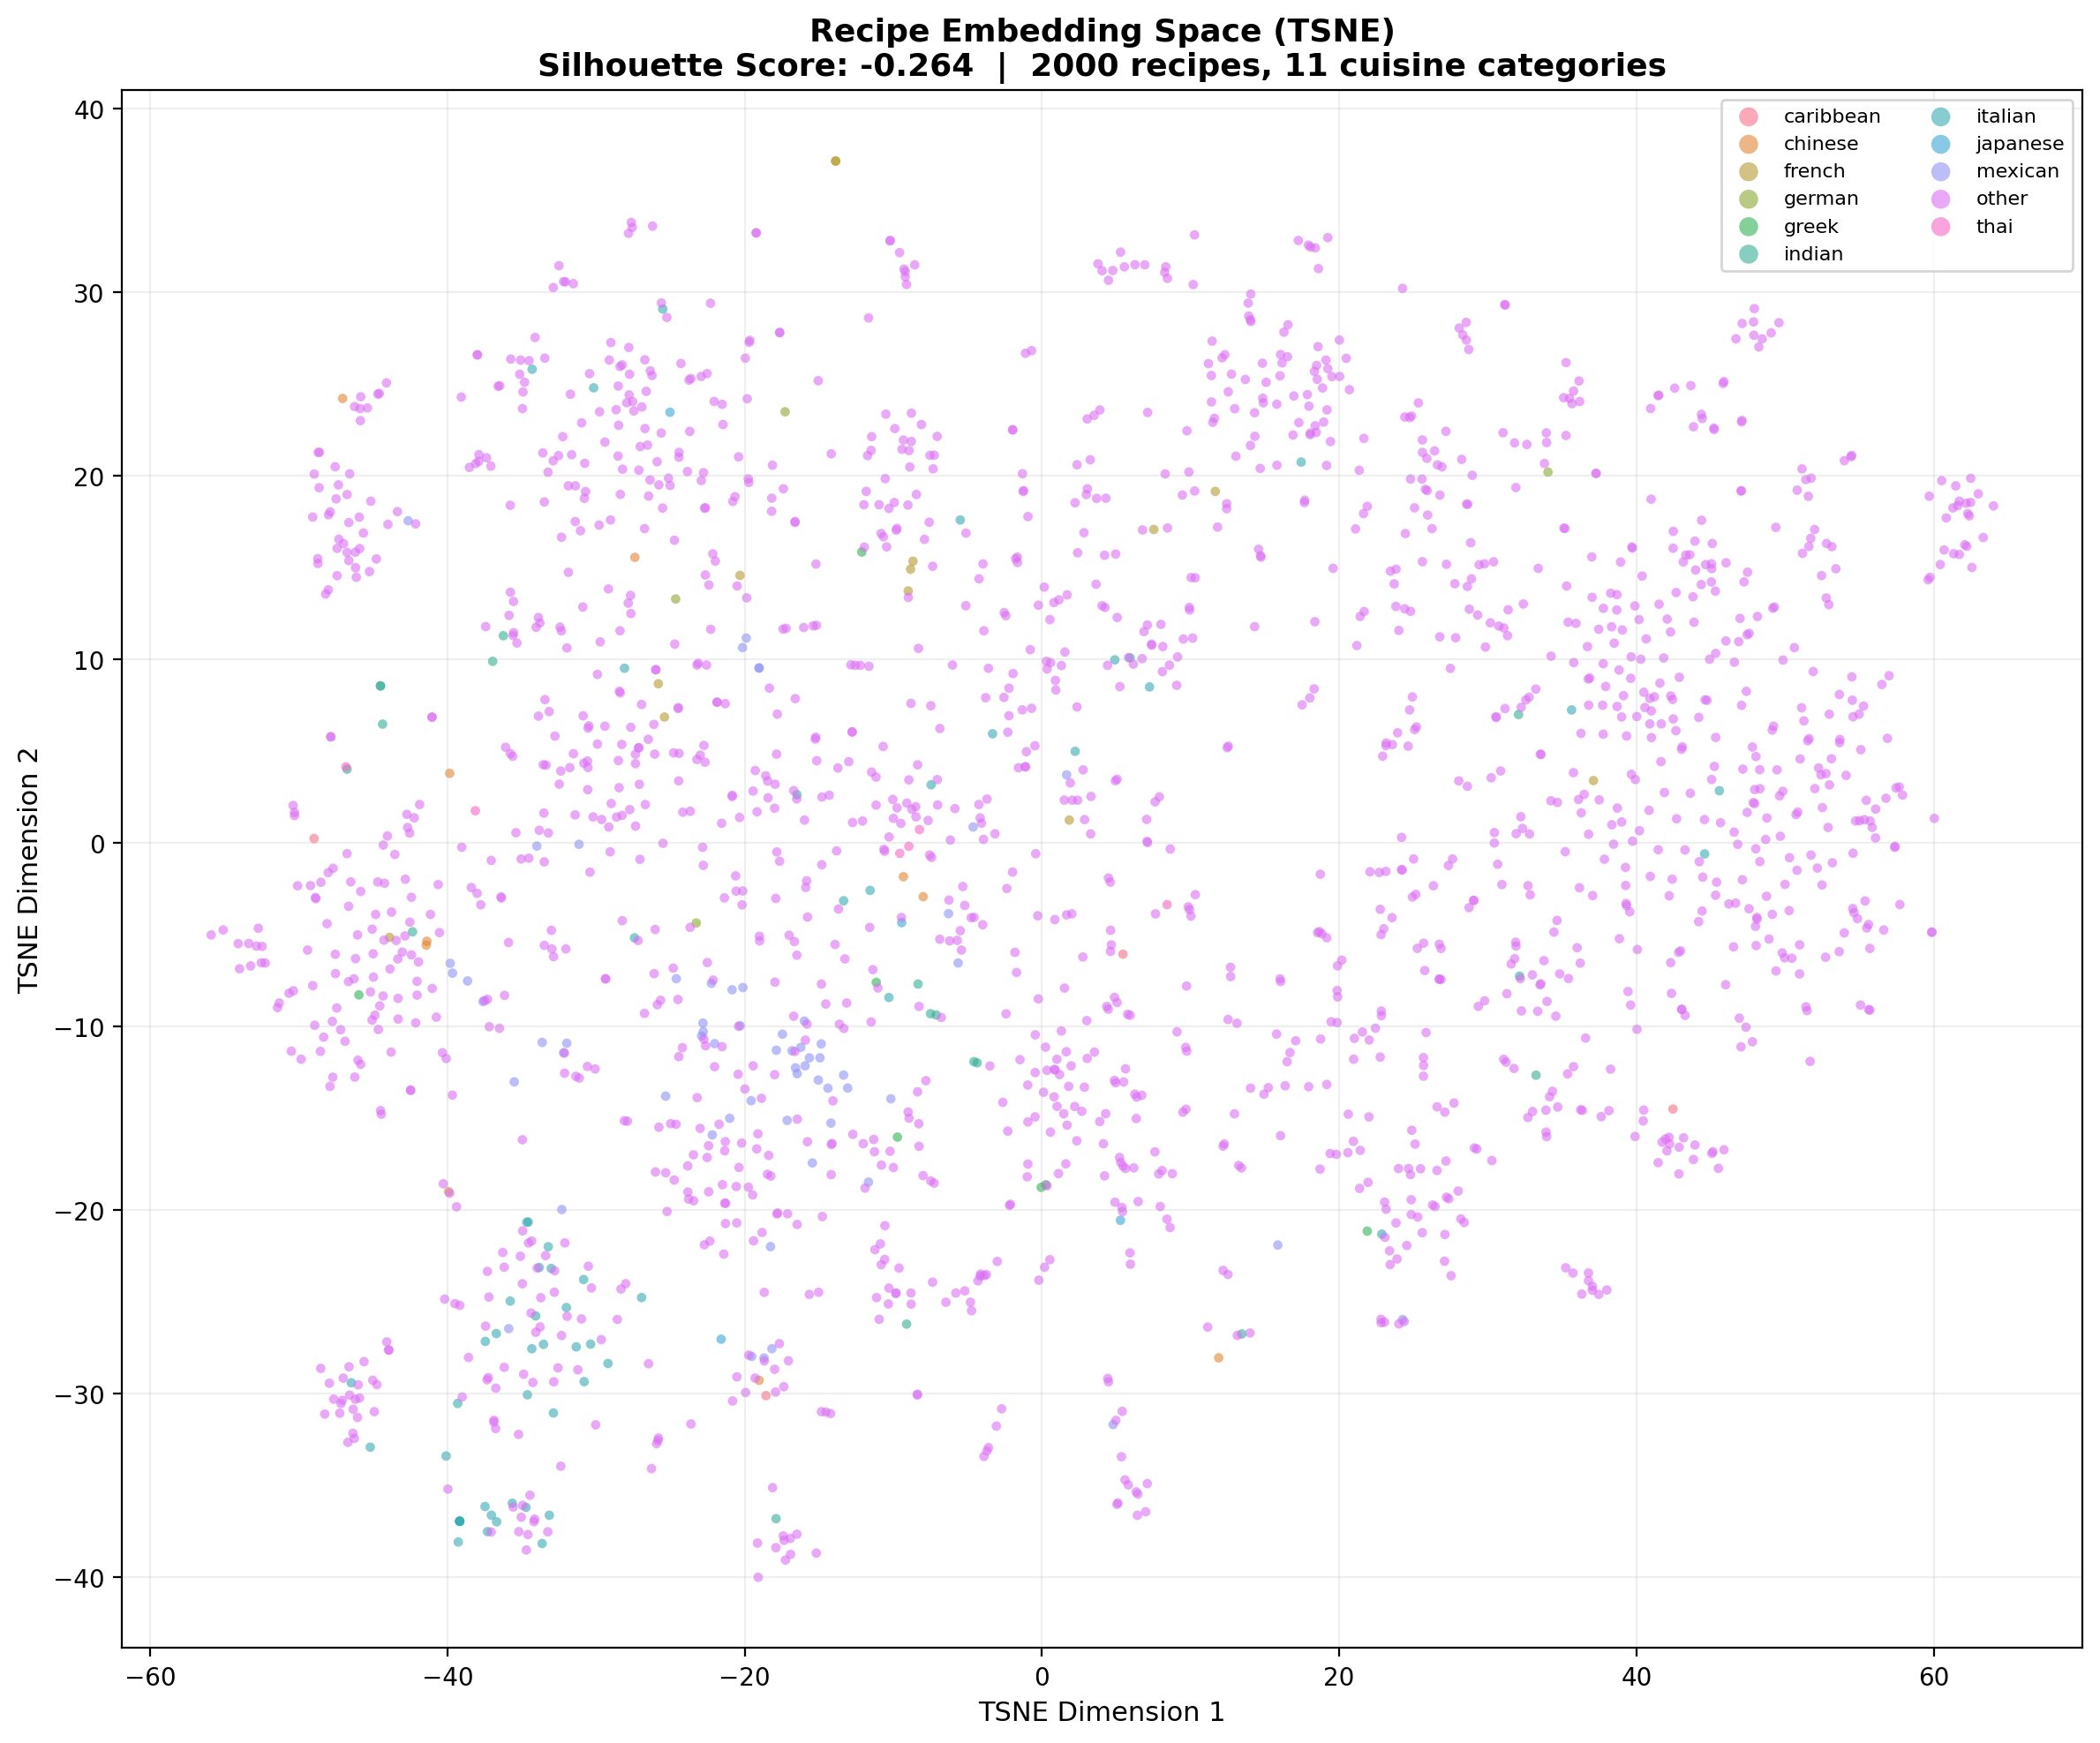
\includegraphics[width=\columnwidth]{embedding_space_tsne.png}
\caption{t-SNE visualization of recipe embeddings colored by cuisine tag. Silhouette score: $-0.264$, indicating weak cuisine-based clustering.}
\label{fig:embedding}
\end{figure}

The negative silhouette score ($-0.264$) reveals that recipe embeddings do not form distinct cuisine-based clusters. This is expected: recipe preparation steps (the indexed text) share vocabulary across cuisines (e.g., ``saut\'{e},'' ``simmer,'' ``season''). This finding motivates the hybrid approach, as BM25 can match explicit cuisine tags that the embedding space fails to separate, while the knowledge graph captures cuisine-ingredient relationships that are lost in the embedding.

% ============================================================
\section{Correctness Verification}

\subsection{Test Suite Overview}

We implemented a comprehensive pytest test suite with 146 tests across 11 test modules, covering all system components:

\begin{table}[H]
\centering
\caption{Test suite breakdown by module (146 total tests, all passing).}
\label{tab:tests}
\small
\begin{tabular}{@{}lcp{4cm}@{}}
\toprule
\textbf{Module} & \textbf{Tests} & \textbf{Scope} \\
\midrule
test\_json\_utils & 12 & JSON extraction from LLM output \\
test\_metrics & 22 & Pipeline evaluation metrics \\
test\_retrieval\_metrics & 21 & IR metrics (P@k, R@k, MRR, NDCG, MAP) \\
test\_critic & 8 & Critic rule-based checks \\
test\_allergy\_checker & 14 & Allergen detection (aliases, API) \\
test\_grocery\_list & 12 & Categorization, dedup \\
test\_nutrition & 9 & PDV conversion, summation \\
test\_budget\_estimator & 7 & Price matching, totals \\
test\_memory\_store & 11 & SQLite persistence \\
test\_knowledge\_graph & 12 & Graph ops, reranking \\
test\_pipeline & 6 & Integration (mocked LLM) \\
\midrule
\textbf{Total} & \textbf{146} & \\
\bottomrule
\end{tabular}
\end{table}

\subsection{Component-Level Testing}

Key verification areas:
\begin{itemize}[nosep]
    \item \textbf{IR Metrics}: Verified precision@k, recall@k, MRR, NDCG@k, and MAP against hand-computed expected values with known retrieval orderings
    \item \textbf{Allergy Checker}: Tested 8 allergen categories (peanuts, dairy, gluten, soy, eggs, shellfish, tree nuts, fish) with alias expansion and case-insensitive matching
    \item \textbf{Knowledge Graph}: Verified graph construction (correct node/edge counts), related recipe discovery, and preference-aware re-ranking
    \item \textbf{Memory Store}: Write/retrieve round-trips, user isolation, preference updates, and session counting using temporary SQLite databases
\end{itemize}

\subsection{Integration Testing}

Six integration tests verify the full pipeline with a mocked LLM client:
\begin{itemize}[nosep]
    \item Pipeline produces valid AgentResult with recipes, grocery list, nutrition
    \item Tool calls are logged correctly
    \item Allergen checking runs for each recipe
    \item Memory context is injected into the planner prompt
\end{itemize}

All 146 tests pass in 7 seconds with no external dependencies (no API keys or Ollama required).

% ============================================================
\section{Web Application}

The system provides a Streamlit web interface with six functional tabs:

\begin{enumerate}[nosep]
    \item \textbf{Meal Plan}: Weekly recipes with ingredients, citations, allergy status, and PDF download
    \item \textbf{Grocery \& Budget}: Categorized ingredient list with estimated costs and pie chart breakdown
    \item \textbf{Nutrition}: Bar chart of weekly nutrient totals
    \item \textbf{Schedule}: Cooking schedule with drag-and-drop reordering
    \item \textbf{Agent Trace}: Full pipeline trace showing planner prompts, LLM responses, tool call distribution, and critic results
    \item \textbf{Memory}: Learned preferences, recent plans, and per-recipe feedback interface
\end{enumerate}

The UI supports both natural language input (parsed by the LLM) and structured constraint entry (sliders and text fields). An audio input option allows voice-based meal requests. Sample requests are provided for quick demonstration.

\begin{figure}[H]
\centering
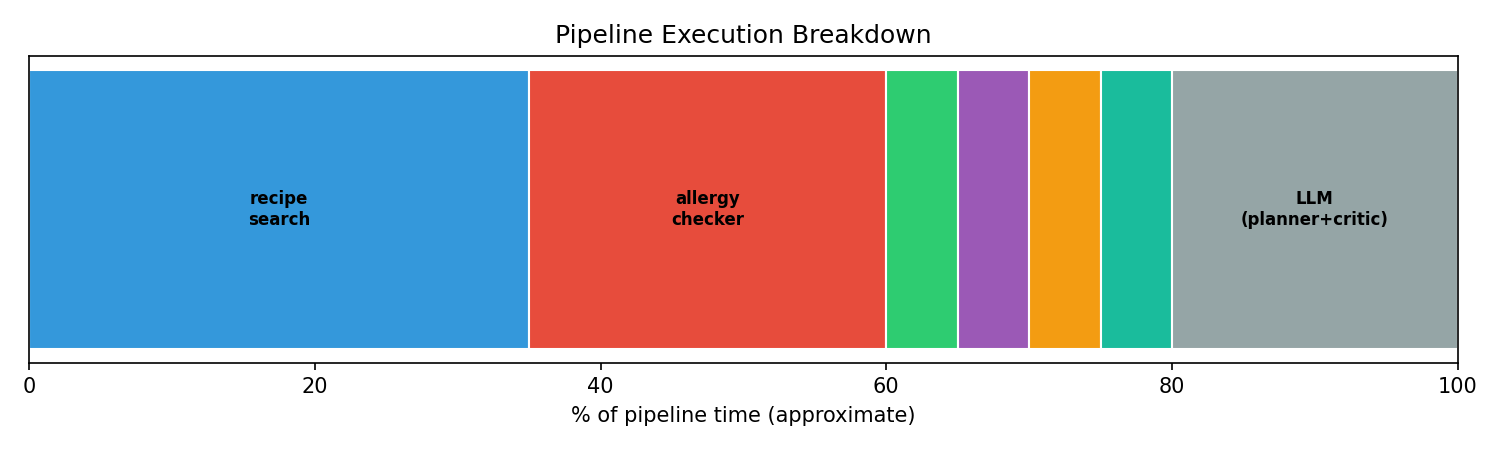
\includegraphics[width=\columnwidth]{pipeline_breakdown.png}
\caption{Pipeline execution time breakdown. Recipe search (RAG) and allergy checking dominate execution time.}
\label{fig:pipeline_breakdown}
\end{figure}

% ============================================================
\section{Discussion}

\subsection{Key Findings}

\textbf{Hybrid retrieval outperforms individual components.} The full hybrid achieves 14\% higher P@5 than BM25 alone and 157\% higher than vector alone. The knowledge graph provides a consistent but modest boost (3--5\% on MRR), while BM25 is the strongest individual component for this domain.

\textbf{Smaller models are viable for structured tasks.} The 2B-parameter Granite model achieves 95\% critic validity, only 5\% below the 70B Llama model. The Planner-Executor-Critic architecture compensates for weaker LLMs through retry-based self-correction.

\textbf{Recipe embeddings do not cluster by cuisine.} The negative silhouette score motivates hybrid retrieval: dense embeddings capture preparation-level similarity, while BM25 and KG capture categorical attributes.

\subsection{Limitations}

\begin{itemize}[nosep]
    \item Gemini evaluation was limited by free-tier quotas; a paid-tier evaluation would complete the model comparison
    \item The knowledge graph uses simple ingredient-overlap similarity; more sophisticated relation extraction could improve KG-based recommendations
    \item The allergy checker relies on string matching and Open Food Facts labels, which may miss cross-contamination risks
    \item Evaluation ground truth is derived from the dataset itself (no human relevance judgments)
\end{itemize}

\subsection{Future Work}

\begin{itemize}[nosep]
    \item Fine-tuning a small LLM on meal planning data to improve plan quality for local models
    \item Incorporating user interaction data for collaborative filtering
    \item Adding nutritional optimization (macro/calorie targets as hard constraints)
    \item Deploying as a production web service with user authentication
\end{itemize}

% ============================================================
\section{Conclusion}

We presented MealPlanAgent, a comprehensive AI meal planning system that combines hybrid retrieval-augmented generation with a Planner-Executor-Critic agent architecture. Our evaluation demonstrates that: (1) the full hybrid retrieval pipeline (BM25 + vector + KG) significantly outperforms individual components, (2) the agent architecture enables reliable meal planning across models ranging from 2B to 70B parameters, (3) stateful memory improves personalization across sessions, and (4) rigorous statistical testing confirms the significance of our design choices. The system is accompanied by a Streamlit web application, 146 passing tests, and evaluation results across 60 structured test cases, 330 retrieval ground truth queries, and 6 ablation configurations.

% ============================================================
\bibliographystyle{plainnat}
\begin{thebibliography}{10}

\bibitem{lewis2020rag}
P.~Lewis, E.~Perez, A.~Piktus, F.~Petroni, V.~Karpukhin, N.~Goyal, H.~K{\"u}ttler, M.~Lewis, W.~Yih, T.~Rockt{\"a}schel, S.~Riedel, and D.~Kiela.
\newblock Retrieval-augmented generation for knowledge-intensive NLP tasks.
\newblock In \emph{NeurIPS}, 2020.

\bibitem{edge2024graphrag}
D.~Edge, H.~Trinh, N.~Cheng, J.~Bradley, A.~Chao, A.~Mody, S.~Truitt, and J.~Larson.
\newblock From local to global: A graph RAG approach to query-focused summarization.
\newblock \emph{arXiv:2404.16130}, 2024.

\bibitem{chen2024bge}
J.~Chen, S.~Xiao, P.~Zhang, K.~Luo, D.~Lian, and Z.~Liu.
\newblock BGE M3-Embedding: Multi-lingual, multi-functionality, multi-granularity text embeddings through self-knowledge distillation.
\newblock \emph{arXiv:2402.03216}, 2024.

\bibitem{schick2023toolformer}
T.~Schick, J.~Dwivedi-Yu, R.~Dess{\`i}, R.~Raileanu, M.~Lomeli, L.~Zettlemoyer, N.~Cancedda, and T.~Scialom.
\newblock Toolformer: Language models can teach themselves to use tools.
\newblock In \emph{NeurIPS}, 2023.

\bibitem{yao2022react}
S.~Yao, J.~Zhao, D.~Yu, N.~Du, I.~Shafran, K.~Narasimhan, and Y.~Cao.
\newblock ReAct: Synergizing reasoning and acting in language models.
\newblock In \emph{ICLR}, 2023.

\bibitem{freyne2010recommending}
J.~Freyne and S.~Berkovsky.
\newblock Intelligent food planning: personalized recipe recommendation.
\newblock In \emph{IUI}, pages 321--324, 2010.

\end{thebibliography}

\end{document}
